\chapter{Models with Time--Varying Dynamics for Pandemic A(H1N1) Influenza in Finland}
\label{chap:lna_extensions}

\section{Overview}
\label{sec:lna_extensions_overview}
To this point, we have largely worked with stochastic epidemic models (SEMs) where the transmission dynamics of an outbreak are time--homogeneous. This may be reasonable for short outbreaks in closed, relatively ``well--mixed" populations, and is often an attractive modeling choice as SEMs with static dynamics are easier to interpret and fit. Incidence data typically arise in settings where the outbreak milieu changes with environmental factors, spatio--temporal heterogeneity in the contact patterns of subpopulations as they are exposed, or behavioral responses as awareness of an outbreak increases and wanes. Furthermore, we are often interested in understanding the effects of time--varying interventions, such as vaccination campaigns, on the transmission dynamics. 

In this chapter, we will demonstrate how the LNA and ODE SEM representations can be used to fit models with time--varying dynamics, which we will then use to model the spread of pandemic A(H1N1) influenza in Finland. We will analyze incidence data from two epidemic seasons, described in Section \ref{subsec:flu_description}. Our goals will be to quantify the transmission dynamics of the outbreak, to estimate the true incidence, and to understand what effect a national vaccination campaign had in mitigating the outbreak severity. 

%We will compare models with time--varying and constant dynamics that we fit using the linear noise approximation (LNA) framework developed in Chapter \ref{chap:lna_for_sems}.

\subsection{On the Importance of Allowing for Time--Varying Dynamics}
\label{subsec:tparam_motivation}

A critical aspect of modeling outbreaks over multiple seasons is that we must account for changes in rates of infectious contacts both within, and between, seasons. The decline in transmission at the end of one season may be attributable, in some combination, to stochastic extinction, a decline in the rate of infectious contact, and a reduction in the effective number of susceptible individuals via immunity acquired from natural exposure or vaccination. It is difficult to explain the emergence of the second season without allowing for stochastic reemergence, changes in the force of infection (FOI), or waning immunity. Put another way, it is highly unlikely an outbreak that died off in a population protected by herd immunity would reemerge absent changes in FOI or repletion of susceptibles in the population. 

Before delving into details of how we intend to accommodate time--inhomogeneity in the FOI, we briefly highlight why we should bother. To make the point, we compare results for two SIRS models fit to incidence data from an outbreak with time--varying dynamics. The data were simulated from an SIRS model where the rate of infectious contact varied sinusoidally over the course of two waves (depicted in Figure \ref{fig:sinfoi_tparam_plots}). While both models allowed for loss of immunity, the per--contact infectious rate was held constant in one model, and in the other was allowed to vary in time, with changes penalized via a first order Gaussian Markov random field (GMRF) shrinkage prior (details presented in Sections \ref{sec:flu_tparam_models} and \ref{sec:tparam_motiv_details}). We used the LNA framework developed in Chapter \ref{chap:lna_for_sems} to fit both models. 

Although both models are misspecified vis--a--vis the  data generating model, the model with time--varying FOI was clearly better able to describe the dynamics of the outbreak (Figure \ref{fig:sinfoi_tparam_plots}). Estimates of basic and effective reproduction numbers capture the true basic and effective reproduction numbers throughout both seasons. The model with time--varying FOI is also able to recover the true incidence. In contrast, the model with homogeneous dynamics fails to accurately estimate the basic and effective reproduction numbers between seasons and during the second wave. It also completely fails to capture the incidence during the second wave. Unlike the model with time--varying FOI, the model with constant FOI also fails to recover the hyperparameters governing the outbreak dynamics and sampling process. In particular the mean duration of immunity and case detection rate are important parameters that are poorly estimated (Figure \ref{fig:sinfoi_param_plots}). Finally, the posterior predictive distributions for the model with time--varying FOI are more accurate, and more precise, than posterior predictive distributions for the model with constant FOI (Figures \ref{fig:sinfoi_tparam_plots} and \ref{fig:sinfoi_ppi_comp}).

\begin{sidewaysfigure}[htbp]
	\centering
	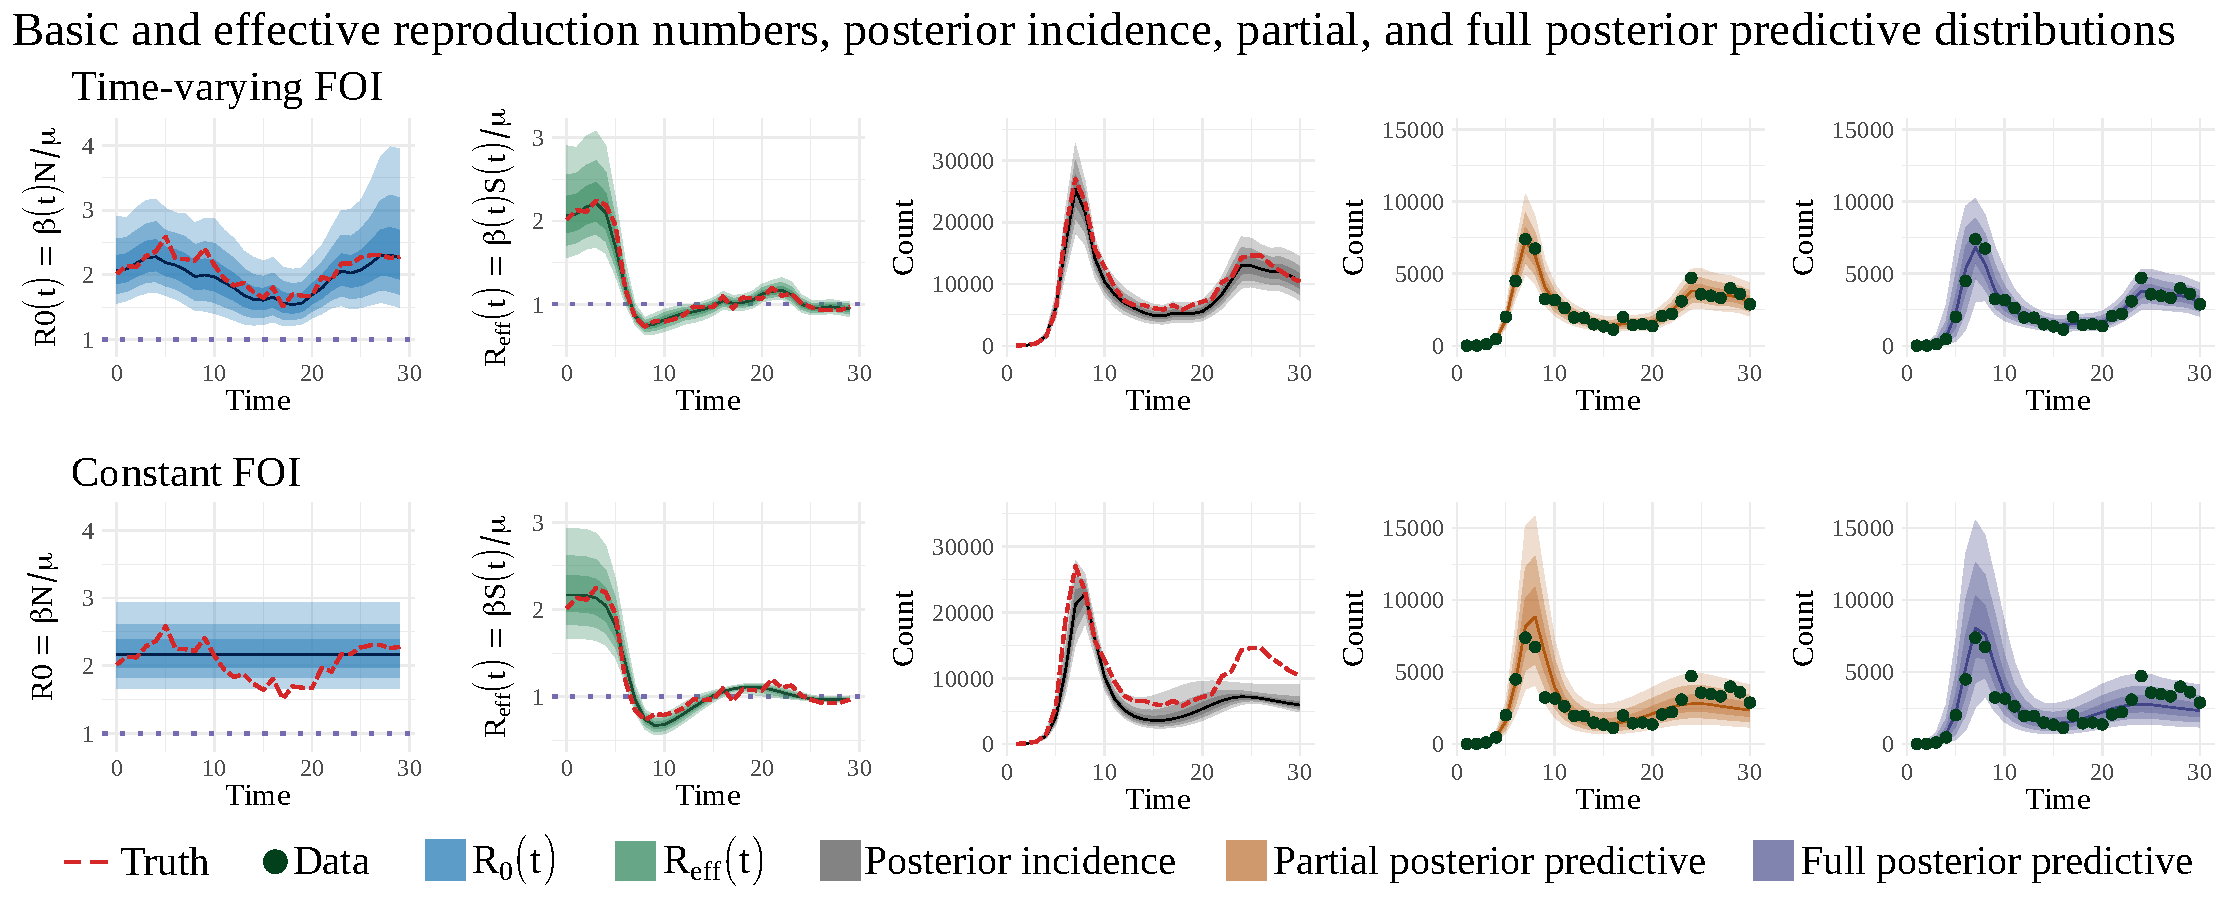
\includegraphics[width=\linewidth]{figures/sinfoi_lna_tparam_plots}
	\caption[Time--varying reproduction numbers, latent incidence, and posterior predictive distributions for SIRS models fit to data from an outbreak with time--varying dynamics.]{Posterior estimates of time--varying quantities. From left to right: basic reproduction numbers, effective reproduction numbers, latent incidence, partial and full posterior predictive distributions. The top row corresponds to estimates obtained using an SIRS model where the basic reproduction number, and hence the per--contact infectivity rate, was allowed to vary in time, with differences penalized according to a first order GMRF. The second row shows estimates obtained from an SIRS model where the per--contact infectivity rate was constant over time. Shaded bands correspond to pointwise 50\%, 80\%, and 95\% Bayesian credible intervals and posterior predictive intervals, with the pointwise posterior/predictive median drawn as a solid line.}
	\label{fig:sinfoi_tparam_plots}
\end{sidewaysfigure}

\begin{figure}[htbp]
	\centering
	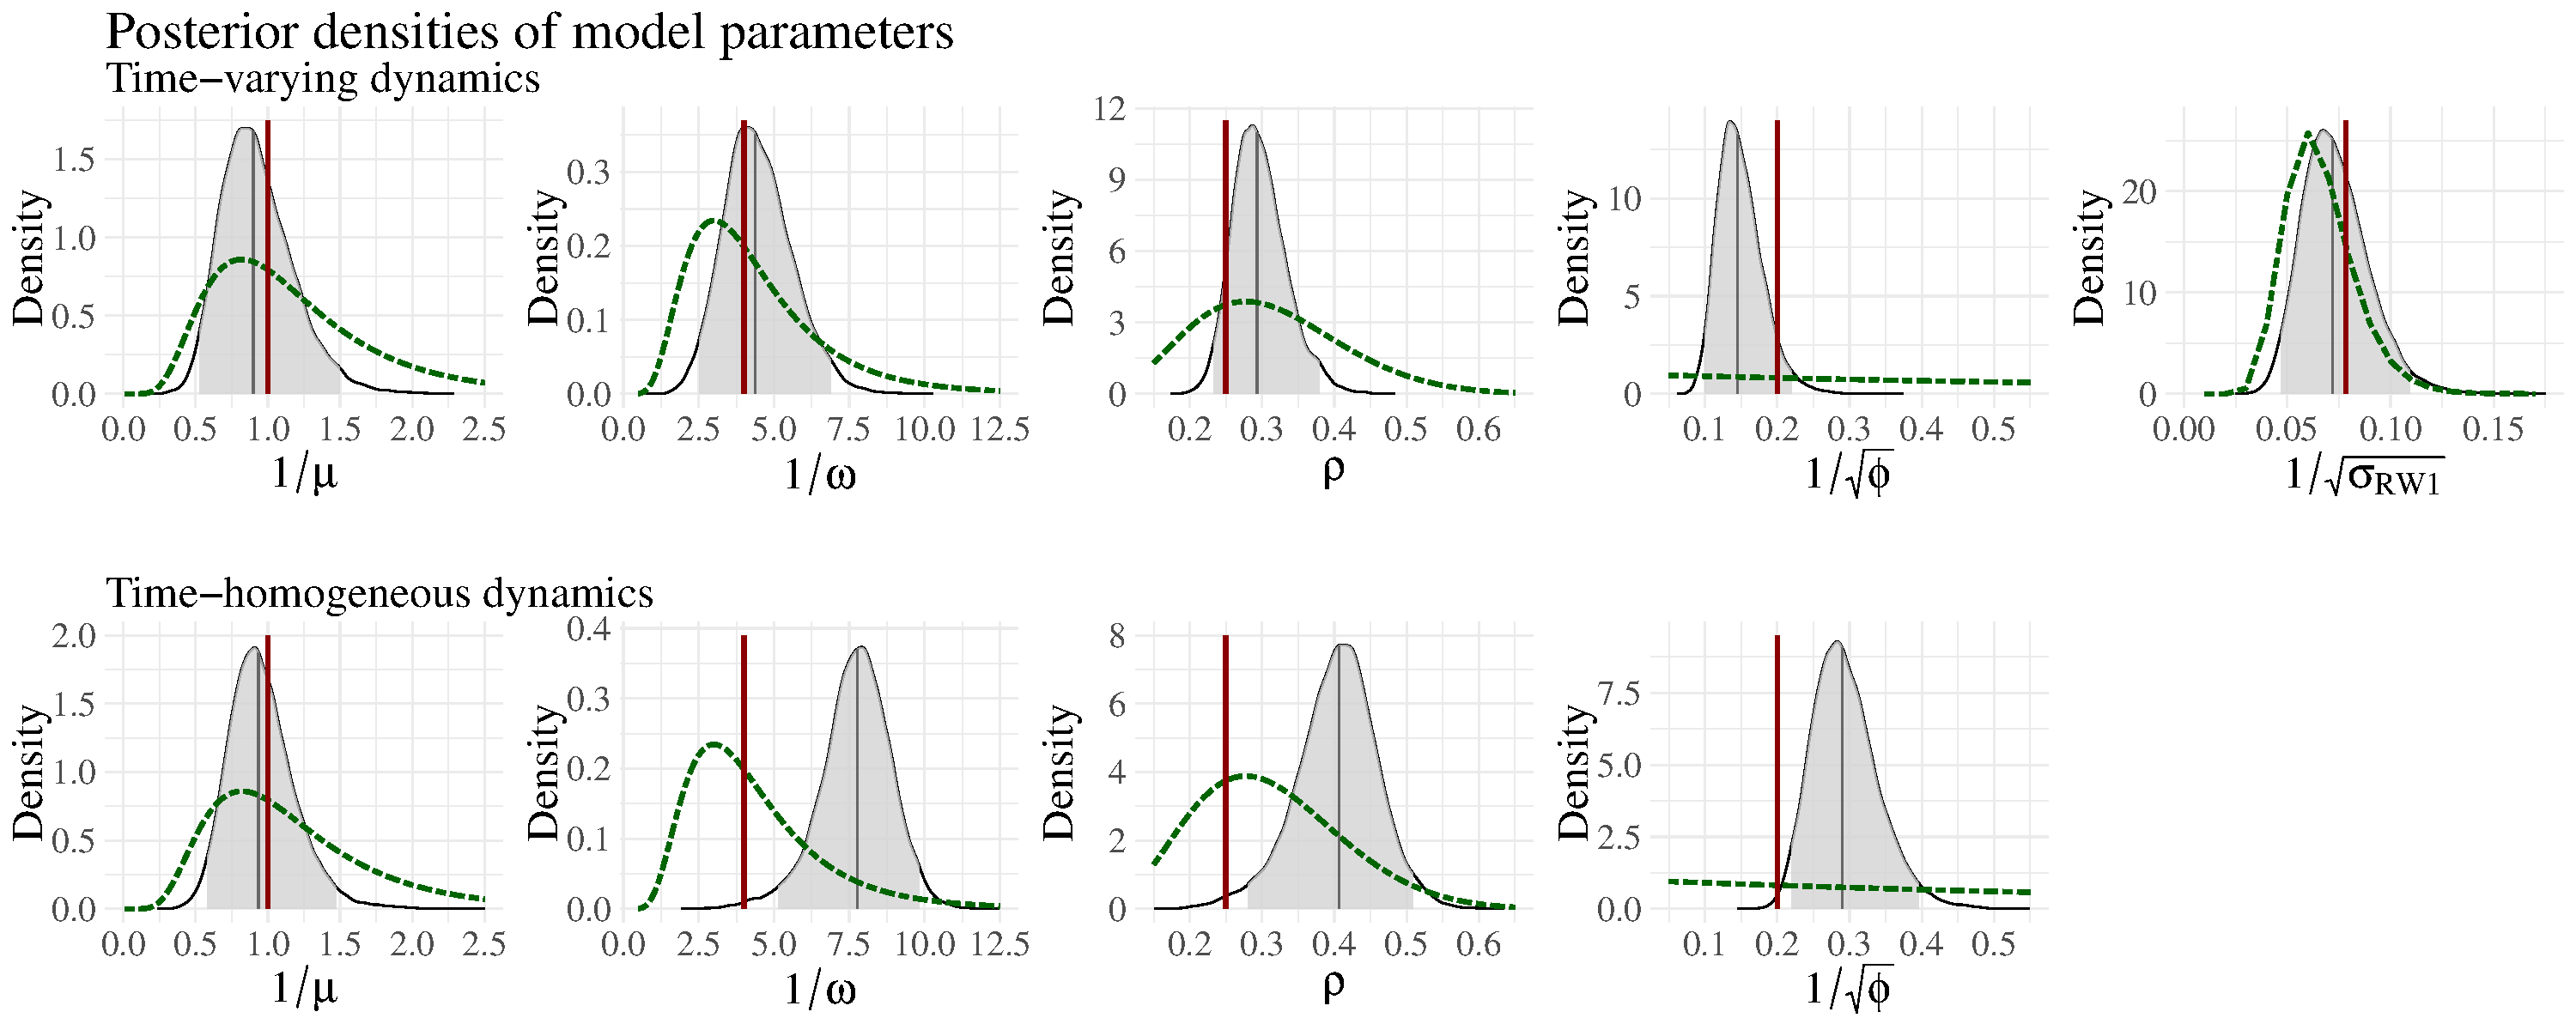
\includegraphics[width=\linewidth]{figures/sinfoi_lna_param_plots}
	\caption[Posterior distributions of SIRS model parameters fit to data from an outbreak with time--varying dynamics.]{Posterior distributions of SIRS model parameters fit to data from an outbreak with time--varying dynamics. From left to right: $ 1/\mu $, the mean infectious period duration; $ 1/\omega $, the mean duration of immunity; $ \rho $, the mean case detection rate; $ \phi $, negative binomial overdispersion parameter; $ \sigma_{GMRF} $, standard deviation of log--differences of time--varying basic reproduction numbers. True values are given by solid red lines and priors by dashed green curves. Solid grey lines are posterior medians, and shaded regions correspond to 95\% Bayesian credible intervals.}
	\label{fig:sinfoi_param_plots}
\end{figure}

\begin{figure}[htbp]
	\centering
	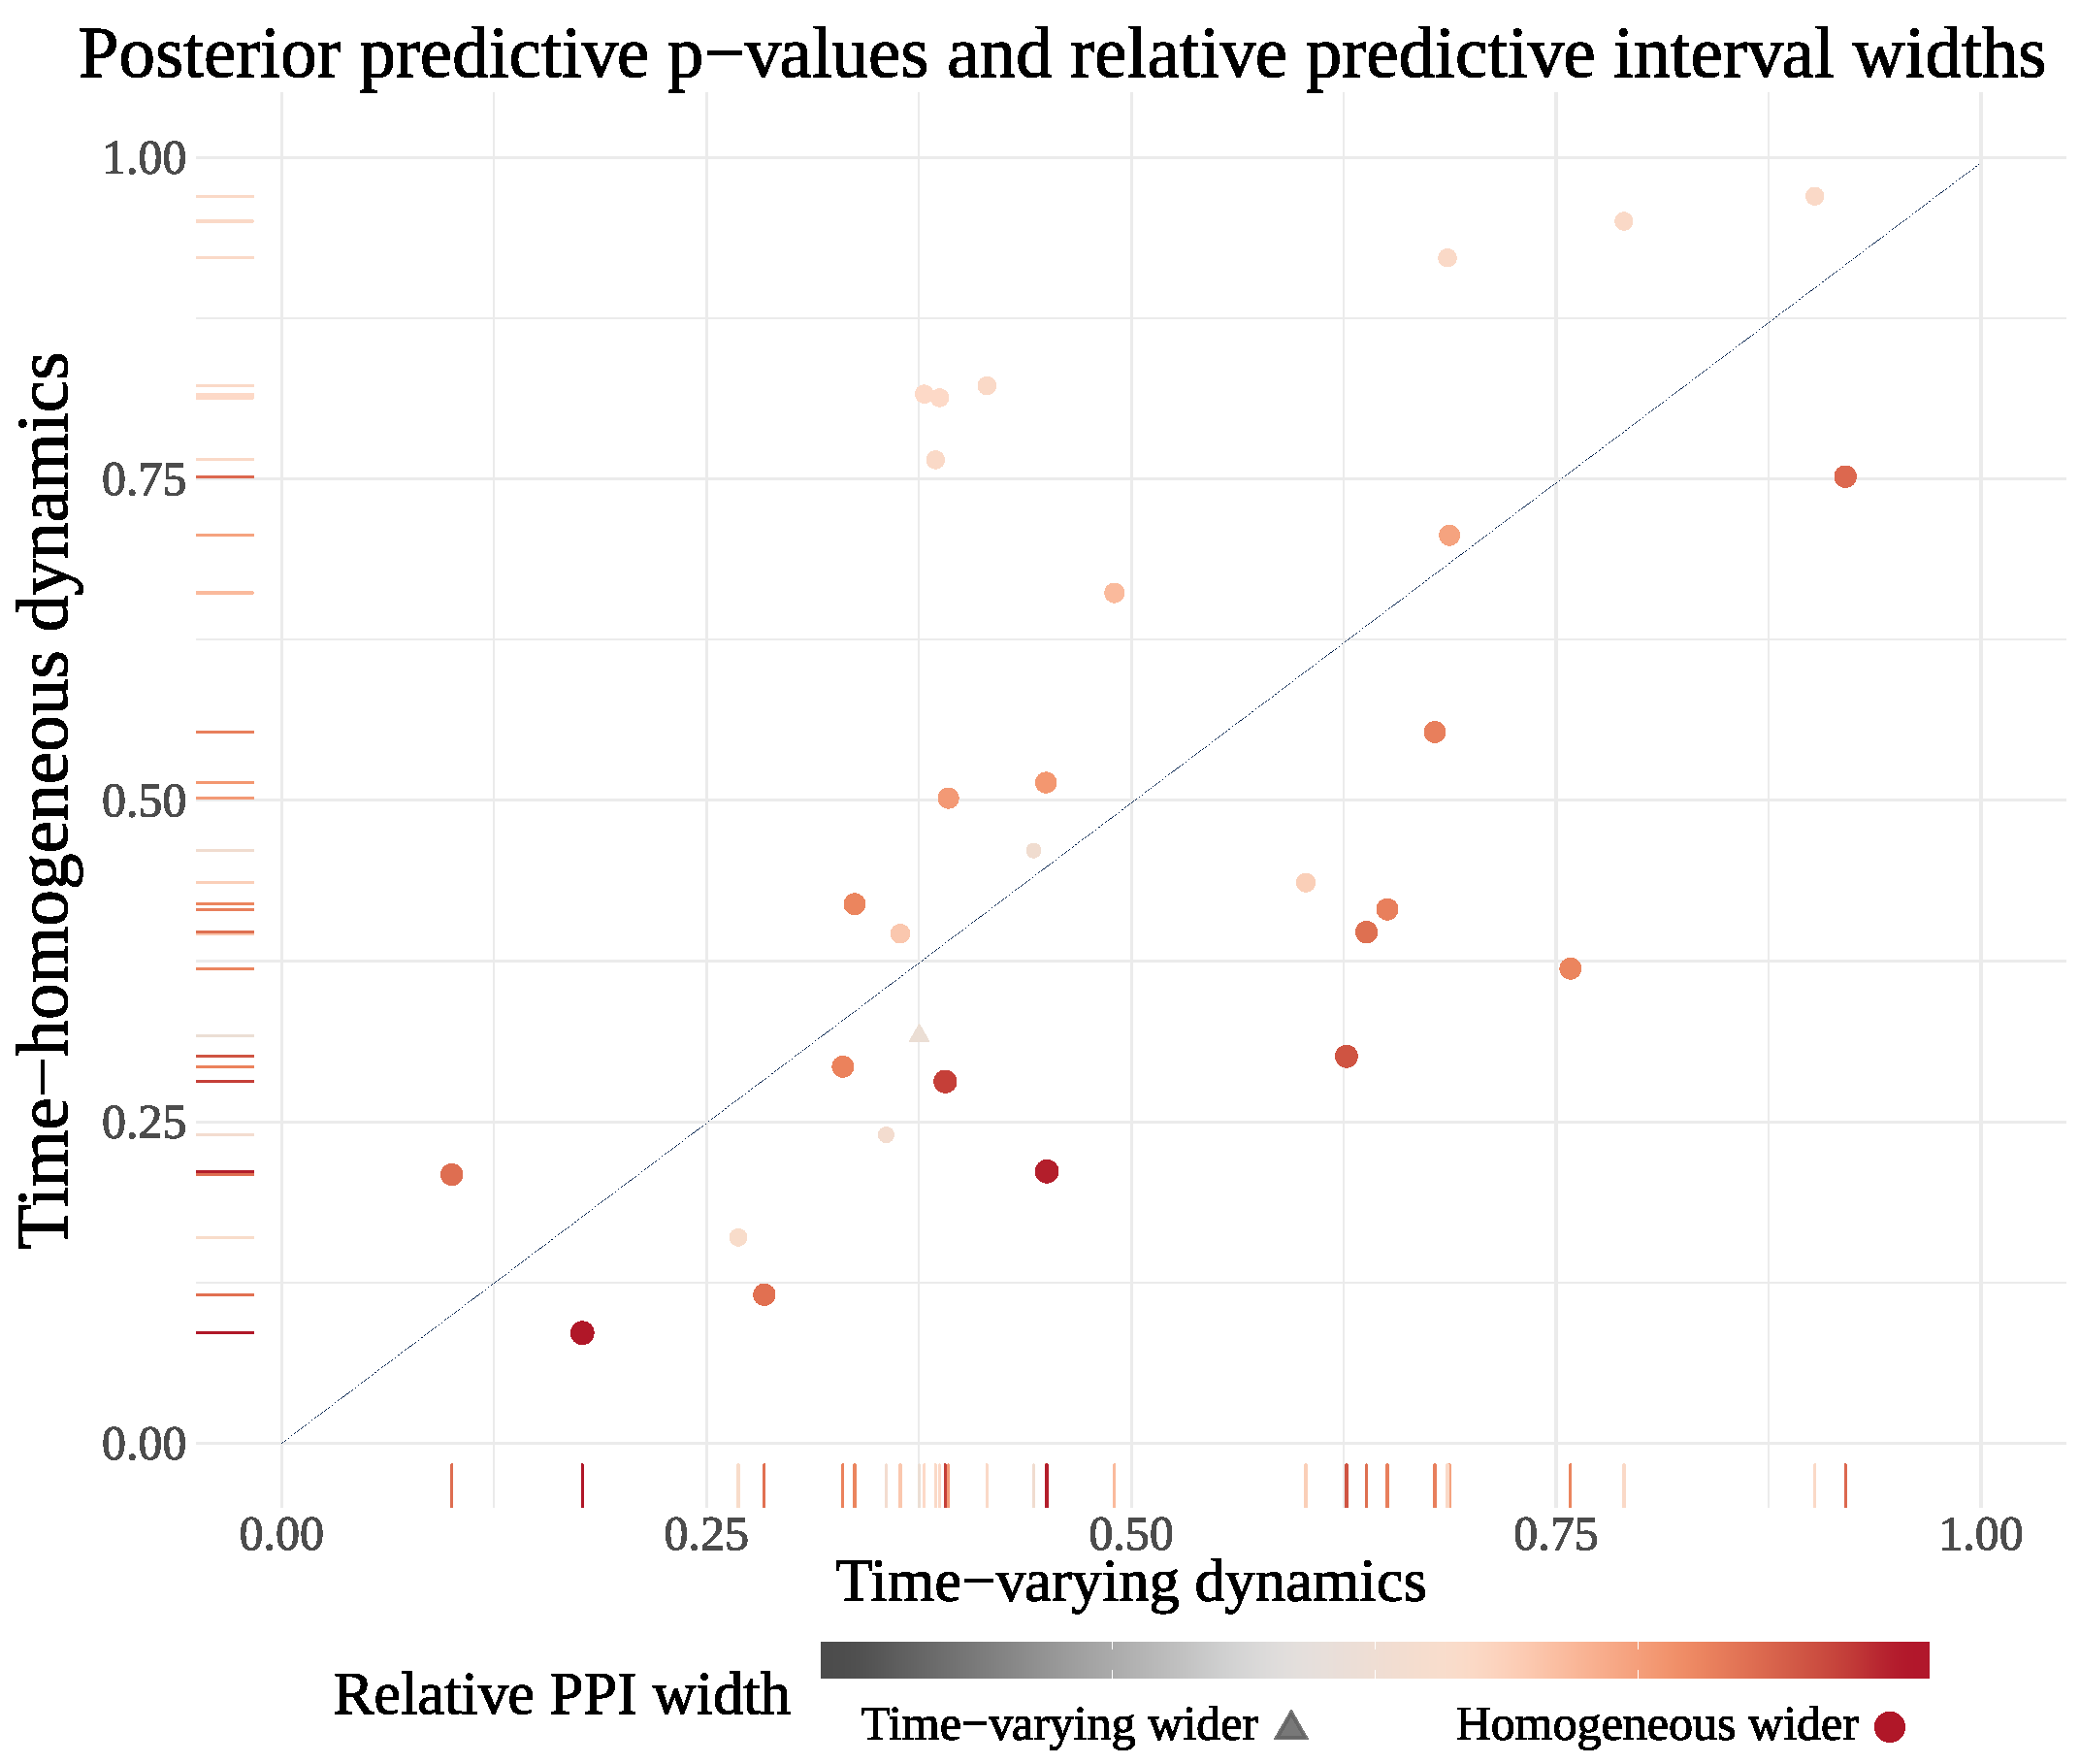
\includegraphics[width=0.8\linewidth]{figures/sinfoi_ppi_comp}
	\caption[Comparison with posterior predictive p-values and relative predictive interval widths for SIRS models fit to an outbreak with time--varying dynamics.]{Comparison of models with time--varying and constant force of infection using posterior predictive p-values (PPPs) and relative posterior predictive interval (PPI) widths. Each point corresponds to the observed incidence in a given week. The X--Y coordinates give the PPPs under time--varying dynamics and time homogeneous dynamics, respectively. The size and color of each point corresponds to the relative PPI width, computed as $ (\widehat{\sigma}_{post,\ell}^{constant} - \widehat{\sigma}_{post,\ell}^{GMRF})/\widehat{\sigma}_{post,\ell}^{GMRF} $, and the sign of the relative width is further emphasized by the shape of the point. Dots indicate that PPIs with constant FOI are wider, the lone triangle corresponds to the one data point where the PPI for the model with time--varying FOI was wider.}
	\label{fig:sinfoi_ppi_comp}
\end{figure}

\newpage
\section{Modeling the Spread of A(H1N1)pdm09 in Finland}
\label{sec:flu_tparam_models}

\subsection{Data and Vaccination}
\label{subsec:flu_datavacc}

We will model the time series of weekly incidence among youths (Y), ages 0--19, and adults (A), ages 20+, over a one year period beginning in epiweek 15, 2009, one month prior to the first observed case in the first season, and a 42 week period beginning in epiweek 33, 2010, corresponding to the start of the 2010--2011 Finnish school year \cite{calendarFinland}. Data from the inter--season period, epiweeks 15--32, 2010, were aggregated over the inter--season period and indexed at epiweek 33, 2010. We denote the data as, $$ \bY = \left (\left (Y_{Y,1},Y_{A,1}\right ),\dots,\left (Y_{Y,52},Y_{A,52}\right ),\left (Y^\prime_{Y,71},Y^\prime_{A,71}\right ),\dots,\left (Y_{Y,113},Y_{A,113}\right )\right ), $$ where the index corresponds to weeks elapsed from week zero, i.e., epiweek 15, 2009. The observed incidence in age--stratum $ j $ at week $ \ell $ is modeled as a negative binomial sample of the true incidence \begin{equation}
\label{flu_emit_prob}
Y_{j,\ell} \sim \mr{Neg.Binom}\left (\mu = \rho_j(\Delta N_{SI}^{(u)}(t_\ell) + \Delta N_{SI}^{(v)}(t_\ell)), \sigma^2 = \mu + \mu^2 / \phi_j\right ),
\end{equation}
where $ \rho_j $ is the age--specific mean case detection rate, $ \phi_j $ is an age--specific overdispersion parameter, and $ \Delta $ is a difference operator for the cumulative incidence in a age--vaccination stratum, e.g., $ \Delta N_{SI}^{(u)}(t_\ell) = N_{SI}^{(u)}(t_\ell) - N_{SI}^{(u)}(t_{\ell-1}) $ is change in cumulative incidence between times $ t_{\ell-1} $ and $ t_\ell $. Three cases, two among adults and one among youths, were detected over the interseason period and were treated as if they were accrued at epiweek 33, 2010. 

\begin{sidewaysfigure}[htbp]
	\centering
	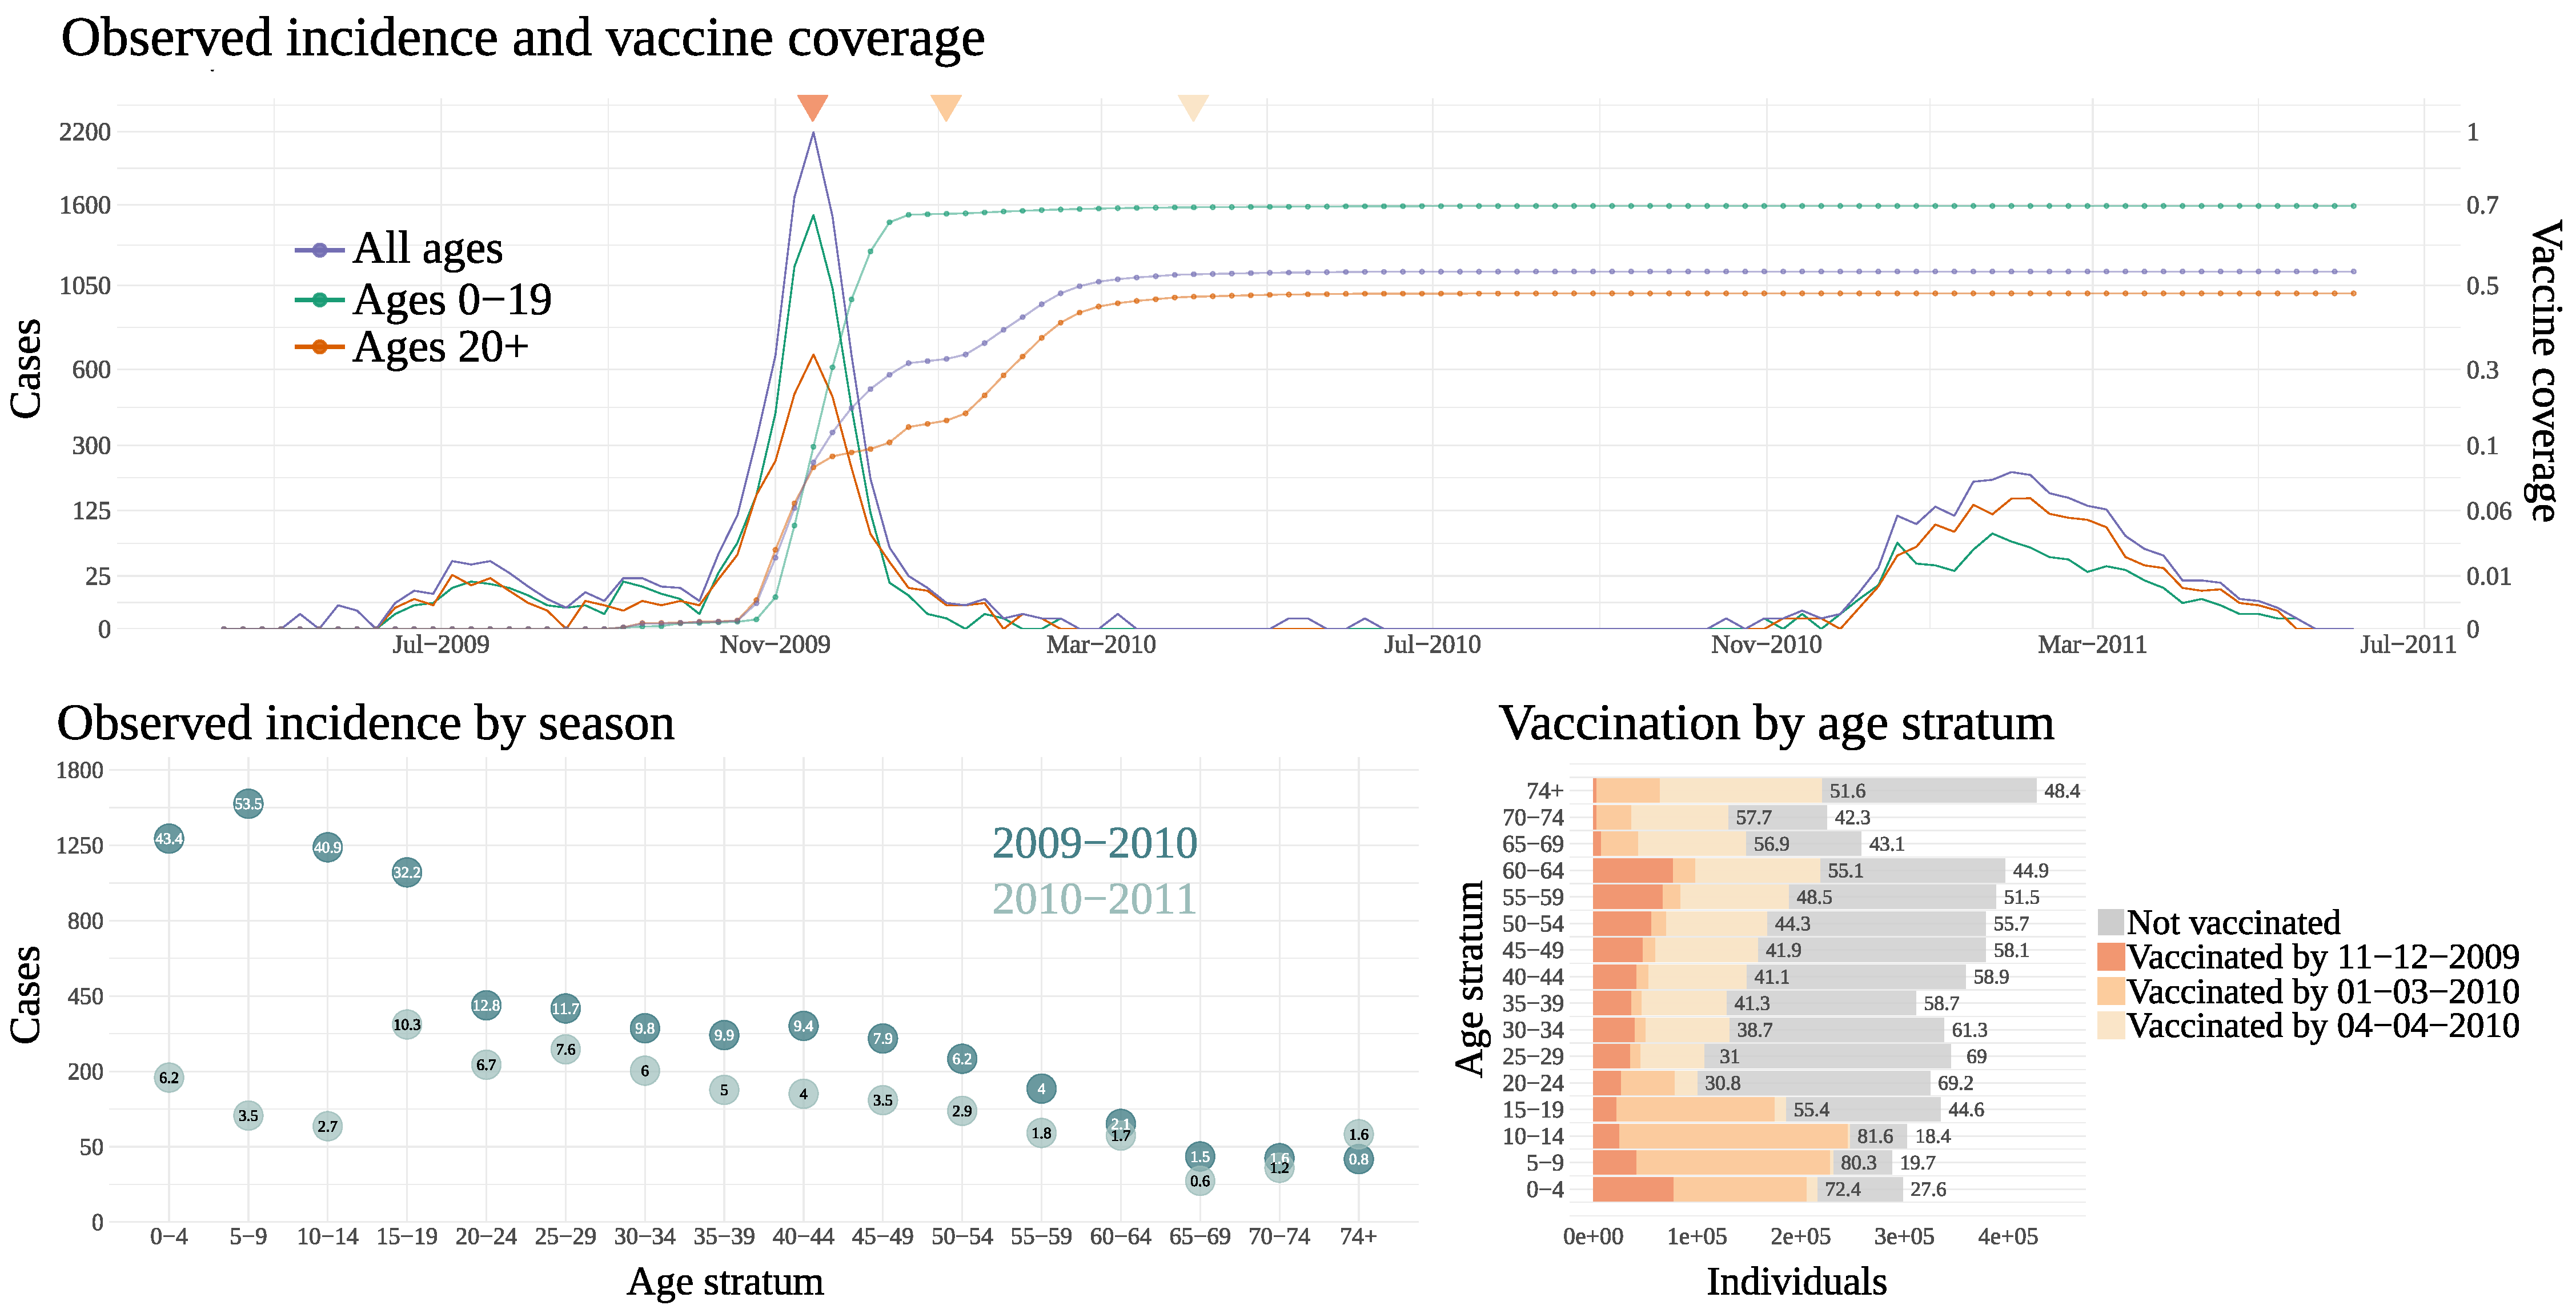
\includegraphics[width=\linewidth]{figures/fludat_plots}
	\caption[A(H1N1)pdm09 incidence and vaccination data from Finland, April 15, 2009 --- June 5, 2011.]{\textbf{Influenza data summaries}. \textit{Top}: Observed incidence (solid lines) and vaccine coverage (lines with points). \textit{Bottom left}: Observed cases by season and age stratum. The 2009--2010 season (dark green) corresponds to the period from April 15, 2009 through April 4, 2010. The 2010--2011 season (light green) corresponds to the period from September 12, 2010 through June 5, 2011. Numbers in points give the attack rate within each stratum for the corresponding season. \textit{Bottom right}: Vaccination coverage by age stratum, colored by vaccine coverages at the times of peak incidence in the first season, tail of the major outbreak in the first season, and end of the vaccination campaign. The numbers inside and outside the histograms denote the percentage of individuals in each stratum that were vaccinated and unvaccinated, respectively, by the end of the vaccination campaign. The times at which vaccine coverages are summarized, denoted by colors of histogram bars, are also identified by corresponding triangles above the top figure.}
	\label{fig:finland_fludat}
\end{sidewaysfigure}

\subsection{Model Structure}
\label{subsec:flu_modstructure}

We fit an age--vaccination stratified susceptible--infected--recovered--susceptible (SIRS) model in which individuals transitioned stochastically, and continuously in time, between disease states. Individuals were assumed to become infectious immediately upon becoming infected, and acquire temporary, though potentially long lasting, protection upon recovery. Individuals who lost immunity were assumed to become fully susceptible. We estimated the initial number of susceptibles as a parameters in the model and assumed that individuals who were not initially susceptible were detached from the transmission processes but could still be vaccinated. The implications of estimating the initial numbers of susceptibles are discussed in Section \ref{subsec:flu_highsusc_sensitivity}. Following \cite{shubin2016revealing}, we assume a closed population and ignore demographic changes or mortality. The model is diagrammed in Figure \ref{fig:flu_sirs_diag}, and Table \ref{tab:flu_notation} lists the model parameters and their interpretations. 

\begin{table}[htbp]
	\caption{Summary of notation for influenza models.}
	\label{tab:flu_notation}
	\footnotesize
	\centering
	\begin{tabular}{llc}
		\hline
		\textbf{Parameter} & \textbf{Interpretation} & \textbf{Time--varying}\\
		\hline
		$\alpha_j(t)$ & Rate of exogenous infectious contact, age stratum $ j $ & Yes \\
		$ \beta_j(t) $ & Per--contact rate of endogenous infection, age stratum $ j $ & Yes \\
		$ \nu $ & Rel. rate of infectious contact for vaccinated ($ 1- $VE for susceptibility) & No \\
		$1/\mu_j$ & Mean infectious period duration, age stratum $ j $ & No\\
		$ 1/\omega $ & Mean duration of immunity & No \\
		$ \rho_j $ & Mean case detection rate, age stratum $ j $ & No\\
		$ \phi_j $ & Negative binomial overdispersion parameter, age stratum $ j $ & No \\
		$ \bX(t) $ & Compartment counts at time $ t $ & Yes\\
		$ \bN(t) $ & Cumulative incidence by time $ t $ & Yes \\
		\hline \hline
		\textbf{Variable} & \textbf{Interpretation} & \textbf{Time-varying}\\
		\hline		
		$ Y_{j,\ell} $ & Observed incidence, age stratum $ j $, time $ t_\ell $ & Yes \\
		$ \mathcal{T} $ & Observation times, numbered by week:  $ \lbrace t_\ell:\ \ell=1,\dots,52,71,\dots,113\rbrace $& No \\
		$ N$ & Population size & No\\
		$ N_{j}^{(k)}(t_\ell) $ & Size of age stratum $ j $ with vaccination status $ k $ in week $ \ell $ & Yes \\
		$ s_{j} $ & Initially susceptible fraction of age stratum $ j $, $ s_j = S_j^{(u)}(t_0) / N_{j}^{(u)}(t_0) $ & No\\ 
		$ V_{j}(t_\ell) $ & \# vaccine doses to individuals in age stratum j at week $ \ell $ & Yes\\	
		$ P^v_{j}(t_\ell) $ & Vaccination coverage in age stratum $ j $ by week $ \ell $ & Yes \\
		$ \xi_{k,j}^{(uv)}(t_\ell) $ & Vaccination forcing for compartment $ k $ in age stratum $ j $ in week $ \ell $ & Yes\\
		$ C_{jk} $ & Relative contact rate to age stratum $ j $ from stratum $ k $ & No\\
		$ R_0(t) $ & Basic reproduction number at time $ t $ & Yes \\
		$ R_{eff}(t) $ & Effective reproduction number at time $ t $ & Yes \\
		$ T_{0,j}(t) $ & Basic type reproduction number at time $ t $, stratum $ j $ & Yes \\
		$ T_{eff,j}(t) $ & Effective type reproduction number at time $ t $, stratum $ j $ & Yes \\
		$ \psi_j(t) $ & Intrinsic reproduction number at time $ t $, stratum $ j $ & Yes\\
		\hline
	\end{tabular}
\end{table}

We take sojourn time in each disease state to be exponentially distributed and leverage the exchangeability of individuals within the model to represent the time--evolution of the epidemic as a Markov jump process (MJP), $$ \bX^c = \left \lbrace S_{Y}^{(u)}, I_{Y}^{(u)}, R_{Y}^{(u)},D_Y^{(u)},
S_{Y}^{(v)}, I_{Y}^{(v)}, R_{Y}^{(v)},D_Y^{(v)}, S_{A}^{(u)}, I_{A}^{(u)}, R_{A}^{(u)},D_A^{(u)}
S_{A}^{(v)}, I_{A}^{(v)}, R_{A}^{(v)},D_A^{(v)} \right \rbrace, $$ where $ S_j^{(k)},\ I_j^{(k)},\ R_j^{(k)},\ D_j^{(k)} $ are the numbers of susceptible, infected, recovered, and detached (susceptible, but not part of the transmission process) individuals in age stratum $ j $ with vaccination status $ k $. The state space of $ \bX^c $, is the set of compartment counts, $ \mcS_X^c$. $ \bX^c $ is also coupled to the cumulative incidence process $ \bN^c $ on the state space of cumulative incidence counts $ \mcS_N^c $, as described in Section \ref{subsubsec:cle_repar}.

\begin{figure}[htbp]
	\centering
	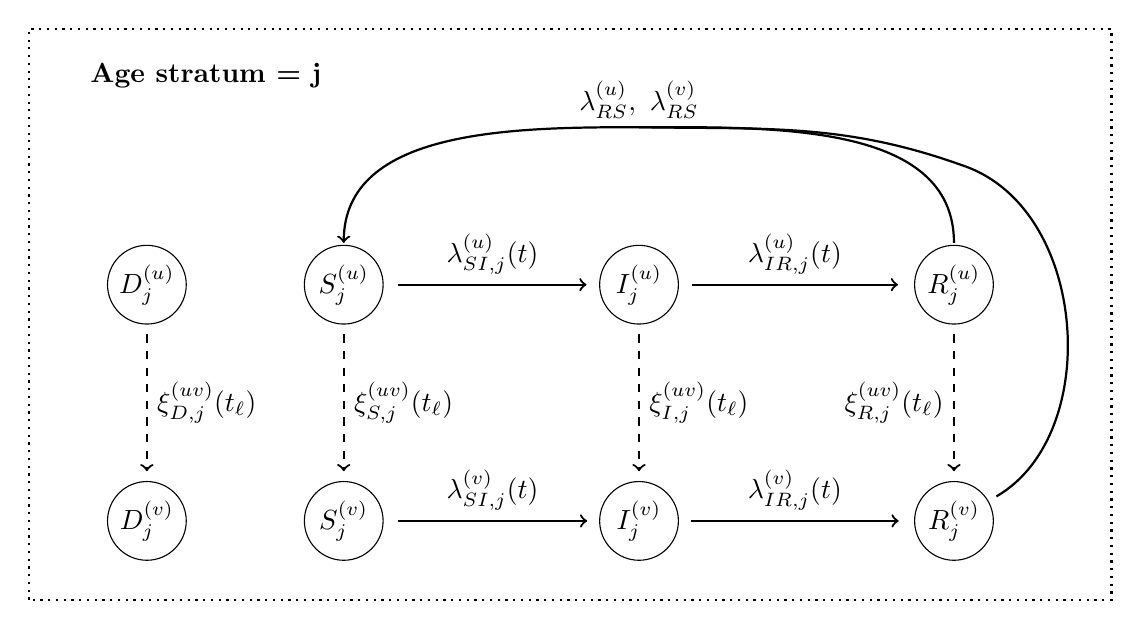
\begin{tikzpicture}
	\draw[thick,dotted] (-2.75,1) rectangle (11,8.25);
	\node at (-0.5,7.25) [label={\textbf{Age stratum = j}}] {};
	\draw (-1.25,5) circle(0.5) node (Dju) {$D_j^{(u)}$};
	\draw (1.25,5) circle(0.5) node (Sju) {$S_j^{(u)}$};
	\draw (5,5) circle(0.5) node (Iju) {$I_j^{(u)}$};
	\draw (9,5) circle(0.5) node (Rju) {$R_j^{(u)}$};
	\draw (-1.25,2) circle(0.5) node (Djv) {$D_j^{(v)}$};
	\draw (1.25,2) circle(0.5) node (Sjv) {$S_j^{(v)}$};
	\draw (5,2) circle(0.5) node (Ijv) {$I_j^{(v)}$};
	\draw (9,2) circle(0.5) node (Rjv) {$R_j^{(v)}$};
	\draw (5,7) coordinate (rec) {};
	\draw (5,7.35) node (reclab) {$ \lambda_{RS}^{(u)},\ \lambda_{RS}^{(v)} $};
	\draw (9.15,6.5) coordinate (rec2) {};
	
	\draw [thick,shorten >=0.25cm,shorten <=0.25cm,->] (Sju) -- (Iju) node[midway,above] {$ \lambda_{SI,j}^{(u)}(t) $};
	\draw [thick,shorten >=0.25cm,shorten <=0.25cm,->] (Iju) -- (Rju) node[midway,above] {$ \lambda_{IR,j}^{(u)}(t) $};
	\draw [thick,shorten >=0.25cm,shorten <=0.25cm,->] (Sjv) -- (Ijv) node[midway,above] {$ \lambda_{SI,j}^{(v)}(t) $};
	\draw [thick,shorten >=0.25cm,shorten <=0.25cm,->] (Ijv) -- (Rjv) node[midway,above] {$ \lambda_{IR,j}^{(v)}(t) $};
	
	\draw [dashed,thick,shorten >=0.25cm,shorten <=0.25cm,->] (Dju) -- (Djv) node[midway,right] {$ \xi_{D,j}^{(uv)}(t_\ell) $};
	\draw [dashed,thick,shorten >=0.25cm,shorten <=0.25cm,->] (Sju) -- (Sjv) node[midway,right] {$ \xi_{S,j}^{(uv)}(t_\ell) $};
	\draw [dashed,thick,shorten >=0.25cm,shorten <=0.25cm,->] (Iju) -- (Ijv) node[midway,right] {$ \xi_{I,j}^{(uv)}(t_\ell) $};
	\draw [dashed,thick,shorten >=0.25cm,shorten <=0.25cm,->] (Rju) -- (Rjv) node[midway,left] {$ \xi_{R,j}^{(uv)}(t_\ell) $};
	
	\draw [thick,shorten >=0cm,shorten <=0.15cm] (Rju) to [out=90, in = 0] (rec);
	\draw [thick,shorten >=0cm,shorten <=0.1cm] (Rjv) to [out=30, in = -20] (rec2);
	\draw [thick] (rec2) to [out=160,in=-1] (rec);
	\draw [thick,shorten >=0.15cm,shorten <=0.0cm,->] (rec) to [out=180, in = 90] (Sju);
	\end{tikzpicture}
	\caption[Diagram of state transitions for an age--vaccination stratified SIRS model for influenza.]{Diagram of state transitions for an age--vaccination stratified SIRS model for influenza in Finland. Both age strata, 0--19 and 20+, have the same compartmental structure. Nodes in circles denote model compartments, which are subscripted with age stratum and superscripted with vaccination status. Solid lines indicate stochastic transitions that occur continuously in time. Rates of disease state transitions, denoted by $ \lambda $, are subscripted with the states from which, and to which, individuals flow and by the age stratum. Superscripts for transition rates indicate vaccination status. Dashed lines represent deterministic forcings from unvaccinated to vaccinated compartments that occur at discrete times. The mass of the forcing at time $ t $, denoted $ \xi(t) $, is subscripted by the compartment and age stratum, and superscripted by the direction of the forcing (unvaccinated to vaccinated).} 
	\label{fig:flu_sirs_diag}
\end{figure}

The contact rate between individuals in age stratum $ j $ and age stratum $ k $, denoted $ C_{jk} $, was based on estimated mean contact rates, appropriately standardized (see Section \ref{sec:flu_contact_rates}), from the Finnish arm of the POLYMOD survey \cite{mossong2008social,polymod} and accessed via the \texttt{socialmixr R} package \cite{funk2018socialmixr}. Sixty percent of contacts in the 0--19 age group were from other individuals age 0--19, while eighty--five percent of the contacts in the 20+ age group were from other adults. The rates, $ \blambda = (\blambda_{Y},\blambda_{A}) $, at which individuals in age--stratum $ j \in \lbrace Y,\ A\rbrace $ transition between disease states are

\begin{equation}\small
\label{eqn:flu_sirs_rates}
\blambda_{j} = \left\lbrace
\begin{array}{ll}
\lambda_{SI,j}^{(u)} = \left [\alpha_{j}(t) + \beta_{j}(t)\left (C_{jk}\left (I_{j}^{(u)} + I_{j}^{(v)}\right ) + (1-C_{jk})\left (I_{k}^{(u)} + I_{k}^{(v)}\right )\right )\right ]S_{j}^{u} \\ 
\lambda_{SI,j}^{(v)} = \nu\left [\alpha_{j}(t) + \beta_{j}(t)\left (C_{jk}\left (I_{j}^{(u)} + I_{j}^{(v)}\right ) + (1-C_{jk})\left (I_{k}^{(u)} + I_{k}^{(v)}\right )\right )\right ]S_{j}^{v}\\
\lambda_{IR,j}^{(u)} = \mu_{j} I_{j}^{(u)} \\
\lambda_{IR,j}^{(v)} = \mu_{j} I_{j}^{(v)} \\
\lambda_{RS,j}^{(u)} = \omega R_{j}^{(u)} \\
\lambda_{RS,j}^{(v)} = \omega R_{j}^{(v)}
\end{array}
\right .
\end{equation}

At weekly intervals, we deterministically force individuals from unvaccinated model compartments to the corresponding vaccinated compartments. Following \cite{shubin2016revealing}, we assume that vaccine doses were distributed proportionally to the number of individuals in each unvaccinated compartment of the corresponding age stratum. In \cite{shubin2016revealing}, it was assumed that vaccination was fully protective with 80\% probability two weeks after administration. Here, we will assume that the vaccine is partially protective in that it reduces the rate at which vaccinated individuals become infected. We do not assume that VE for susceptibility varies by age, and also do not model vaccine efficacy for infectiousness or recovery due to the limited extent of the data. To account for the time required to elicit an immune response, we apply the deterministic forcing at the beginning of week after the time when each dose count was indexed. Suppose that at the end of week $ \ell $ we have $ \bX_j^{(u)}(t_\ell) = \left (S_j^{(u)}(t_\ell),\ I_j^{(u)}(t_\ell),\ R_j^{(u)}(t_\ell),\ D_j^{(u)}(t_\ell)\right ) $ unvaccinated susceptible, infected, recovered, and detached individuals in age stratum $ j $ and $ \bX_j^{(v)}(t_\ell) = \left (S_j^{(v)}(t_\ell),\ I_j^{(v)}(t_\ell),\ R_j^{(v)}(t_\ell),\ D_j^{(v)}(t_\ell\right ) $ vaccinated individuals, and that $ V_j(t_\ell) $ vaccine doses were recorded for stratum $ j $ in that week. We apply the vaccine forcing to the initial state for the following week: 
\begin{align}
\label{eqn:vacc_forcing}
\begin{split}
	\bX_{j}^{(u)}(t_\ell^+) &= \bX_j^{(u)}(t_\ell) - V_j(t_\ell)\frac{\bX_{j}^{(u)}(t_\ell)}{\sum\bX_{j}^{(u)}(t_\ell)}, \\
	\bX_{j}^{(v)}(t_\ell^+) &= \bX_j^{(v)}(t_\ell) + V_j(t_\ell)\frac{\bX_{j}^{(u)}(t_\ell)}{\sum\bX_{j}^{(u)}(t_\ell)}.
\end{split}
\end{align}
Thus, the vaccination forcing affects the initial condition for the period $ (t_\ell,t_{\ell+1}] $, not the state at time $ t_\ell $. 

The diffusion approximation for the MJP is a real--valued process, $ \bX $, that in its infinite population limit evolves as a deterministic system of ODEs. The state space of $ \bX $ is defined in terms of compartment volumes, $ \mcS_X^R $, and with corresponding cumulative incidence process, $ \bN $, with state space $ \mcS_N^R $. Note that the boundary conditions on the state spaces of $ \bX^c $ and $ \bN^c $, and similarly of $ \bX $ and $ \bN $, ensure positivity of compartment counts and monotonicity of cumulative incidence paths, and that the compartment counts each age--vaccination stratum sum to the number of individuals in that stratum, e.g., $ S_{Y}^{(u)}(t) + I_{Y}^{(u)}(t) + R_{Y}^{(u)}(t)+ D_{Y}^{(u)}(t) = N_{Y}^{(u)}(t) $. Due to the complexity of the model, we will rely on the deterministic ODE framework that was explored as a comparitor for the LNA in Chapter \ref{chap:lna_for_sems} to facilitate the computation \ref{chap:lna_for_sems}.  

%As in Chapter \ref{chap:lna_for_sems}, we will use the non--centered parameterization of the restarting LNA of the log--transformed SDE to approximate the time--evolution of $ \bX^c $ and $ \bN^c $. Algorithm \ref{alg:doLNA2} details the procedure for mapping standard normal LNA draws onto an LNA sample path with vaccination forcings.

\subsubsection{Reproduction numbers}
\label{subsubsec:stratmod_repnumbs}
The basic reproduction number, $ R_0 $, and its variants describe the propensity of an outbreak to spread through a population \cite{heffernan2005perspectives,van2008further}. $ R_0 $ is loosely interpreted as the average number of secondary infections arising from a single infected individual in a completely susceptible population. An outbreak will fail to sustain itself (almost surely when it evolves deterministically, but in reality with high probability due to the inherently stochastic nature of epidemics) when $ R_0 < 1 $. For this reason, epidemiologists often quantify the effectiveness of a control measure by estimating the extent to which the intervention reduces $ R_0 $. We can interpret the basic reproduction number as an intrinsic reproduction number when there is an exogenous contribution to force of infection \cite{blackwood2018introduction}. From a modeling perspective, is important to understand not only how $ R_0 $ affects the transmission dynamics, but also how various aspects of the model interact to affect $ R_0 $. 

The basic reproduction number of a structured SEM can be obtained by computing the spectral radius (absolute value of the dominant eigenvalue) of the next generation matrix (NGM) for the linearized system of ODEs specifying the flow in and out of states at infection \cite{heffernan2005perspectives,van2017reproduction,van2008further}. The $ i,j $ element of the NGM gives the expected number of secondary infections in age stratum $ i $ given an index infection in stratum $ j $. Noting that vaccinated and unvaccinated invididuals in this model are equally transmissive and have the same mean infectious period durations, we obtain the age--structured next generation matrix
\begin{align}
\label{eqn:sirs_ngm_full}
\bK &= 
	\left (
	\begin{array}{cc}
	K_{YY} & K_{YA} \\
	K_{AY} & K_{AA}
	\end{array}
	\right ) =\left (
	\begin{array}{cc}
	\frac{C_{YY}\beta_Y\left (N_Y^{(u)} + \nu_YN_Y^{(v)}\right )}{\mu_Y} & \frac{C_{YA}\beta_Y\left (N_Y^{(u)} + \nu_YN_Y^{(v)}\right )}{\mu_A} \\[2ex]
	\frac{C_{AY}\beta_A\left (N_A^{(u)} + \nu_AN_A^{(v)}\right )}{\mu_Y} & \frac{C_{AA}\beta_A\left (N_A^{(u)} + \nu_AN_A^{(v)}\right )}{\mu_A}
	\end{array}
	\right ).
\end{align}
The basic reproduction number is 
\begin{align}
\label{eqn:sirs_R0}
R_0 = \frac{1}{2}\left (K_{YY} + K_{AA}\right ) + \frac{1}{2}\sqrt{(K_{YY} - K_{AA})^2 + 4K_{YA}K_{AY}}.
\end{align}

Note that is possible for the outbreak to persist, i.e., $ R_0 > 1 $,  when the intrinsic reproduction number in one of the strata is below 1, e.g., $ K_{YY} <1$, even though most transmission arises from within--group contacts. However, $ R_0 <$ will be less than 1 if both $ K_{YY} <1 $ and $ K_{AA} <1 $.

Furthermore, the basic reproduction number is greater than the average of intrinsic reproduction numbers, $ K_{YY} $ and $ K_{AA} $, since the second term on the right hand side of (\ref{eqn:sirs_R0}) will typically be positive. Similarly, the variance of $ R_0 $ is also greater than the average of variances of $ K_{YY} $ and $ K_{AA} $. For these reasons, we should consider how $ K_{YY} $ and $ K_{AA} $ interact to induce a prior over $ R_0 $ when parameterizing the model. Note that if the cross--stratum contact rates were negligible, $ R_0 $ would behave like the average of intrinsic reproduction numbers plus a term proportional to the absolute difference between $ K_{YY} $ and $ K_{AA} $. This suggests that prior information about the intrinsic reproduction numbers, either individually (our preference) or about their average and difference, could help identify $ R_0 $. We should also keep in mind that our model is more complicated since the cross stratum terms are not negligible ($ C_{AA} = 0.6 $, $ C_{YY}=0.85 $), hence
\begin{align*}
K_{YA} &= \frac{(1 - C_{YY})}{C_{YY}}\frac{\mu_Y}{\mu_A}K_{YY},\hspace{0.25in}
K_{AY} = \frac{(1 - C_{AA})}{C_{AA}}\frac{\mu_A}{\mu_Y}K_{AA},\\
&\implies K_{YA}K_{AY} = \frac{(1 - C_{YY})(1-C_{AA})}{C_{YY}C_{AA}}K_{YY}K_{AA}.
\end{align*} 
Thus, $ R_0 $ is the average of $ K_{YY} $ and $ K_{AA} $, plus a non--linear function of $ K_{YY} $ and $ K_{AA} $.

Finally we emphasize the importance of accounting for all of the parameters that contribute the intrinsic reproduction numbers, and by extension $ R_0 $, when specifying priors and parameterizing the estimation scale of the MCMC. In particular, it is critical to note that the effective population size might be lower than the nominal population size because of vaccination and depletion of susceptibles. We can easily misspecify the scales of prior distributions for the reproduction numbers, or select an inefficient parameterization for the MCMC estimation scale, by neglecting this dynamic. In our model, for example, the value of $ R_0 $ in the first season, and the rate at which recovered individuals lose immunity, will affect the effective population size at the beginning of the second season. 

\subsection{Flexible Models for the Force of Infection with Gaussian Markov Random Fields}
\label{subsec:flu_gmrf}

We will model the time--varying force of infection using first order GMRFs for the log intrinsic reproduction numbers and the effective rate of exogenous infectious contacts in each age stratum. The GMRFs are separately specified over three epochs corresponding to the period one month before the first detected case until the start of the Finnish school year in 2009, the beginning of the Finnish school year in 2009 until its start in 2010 (including the inter--season period), and the second epidemic season beginning at the start of the Finnish school year, 2010. These epochs correspond to epiweeks 15, 2009 through epiweek 34, 2009, epiweek 35, 2009 through epiweek 32, 2010, and epiweek 33, 2010 through epiweek 22, 2011. We will assume that the intrinsic reproduction numbers are homogeneous over the inter--season period, from epiweek 16, 2010 -- epiweek 32, 2010.

Let $ \bpsi_{j} = \lbrace\psi_{j,\ell}:\ \ell \in 0,\dots,52,71,\dots,112\rbrace $ be the vector of intrinsic reproduction numbers for stratum $ j \in \lbrace Y,A \rbrace$, ignoring the relative contact rates, $ C_{jk} $, and vaccination. The reproduction number in time interval $ \ell $, indexed in weeks from epiweek 15, 2009, is
\begin{equation}
\label{eqn:R0t_novacc}
\psi_{j,\ell} = \frac{\beta_j(t_\ell)N_js_j}{\mu_j},
\end{equation}
where $ \beta_j(t_\ell) $ is the per--contact infection rate, $ \mu_j $ is the recovery rate, $ N_j $ is the size of the age stratum, and $ s_j $ is the fraction of individuals in stratum $ j $ that are susceptible.
 
When transmission is sustained at near--endemic levels, we should expect that the effective reproduction numbers are near one, or perhaps slightly above. Let $ \nu $ be the relative rate of infectious contact among vaccinated individuals, i.e., one minus the vaccine efficacy for susceptibility. The effective reproduction number, which accounts for the effects of vaccination and depletion of susceptibles, is 
\begin{equation}
\label{eqn:Reff_t}
\psi_{j,\ell}^{eff} = \frac{\beta_j(t_\ell)_j\left (S^{(u)}_j(t_\ell) + S^{(v)}_j(t_\ell)\nu\right )}{\mu_j}
\end{equation}
If vaccination does not increase the rate of infectious contact (and we will assume it does not), then $ \psi_{j,\ell}^{eff} < \psi_{j,\ell} $ since $ \nu\in[0,1] $ and $ (S^{(u)}_j(t_\ell) + S^{(v)}_j(t_\ell) < N_js_j $. It is critical to account for this when specifying priors for the basic intrinsic reproduction numbers at the start of each epoch. It would not do, for instance, to set priors for the intrinsic basic reproduction numbers at the beginning of the third epoch that nominally concentrate mass near one since this would imply that the effective reproduction numbers are far below one due to vaccination and depletion of susceptibles during the first wave of the outbreak. Our approach will be to assign priors to the vaccination adjusted intrinsic reproduction numbers at the beginning of each epoch, $ \psi_{j,\ell}^\prime = \psi_{j,\ell}  \left (1 - P^v_j(t_\ell) + \nu P^v_j(t_\ell)\right ) $, where $ P_j^v(t_\ell) $ is the vaccination coverage in stratum $ j $ at $ t_\ell $, $ \ell = 0,19,71 $. 

We denote by $ \Delta $ the first--order forward difference operator, i.e., $ \Delta X_j = X_{j+1} - X_j $. The first--order differences of the log intrinsic reproduction numbers for stratum $ j $ in each epoch are assigned a Gaussian prior with mean zero and variance $ \sigma^2_{j,\ell} $. The sub--model for intrinsic reproduction numbers in stratum $ j $ is

\begin{footnotesize}
	\begin{align}
	\log(\psi_{j,\ell}) &\sim \mcN(\mu_{j,\ell},\tau_{j,\ell}^2),&\ &\ell= 0,19,71, \nonumber\\
	\log(\sigma_{j,\ell}) &\sim \mcN(m_{j,\ell}, s_{j,\ell}^2),&\ &\ell=0,19,71, \nonumber\\
	\Delta\log(\psi_{j,\ell})&\sim \mcN(0, \sigma^2_{j,0}),&\ &\ell=0,\dots,17, \nonumber\\
	\Delta\log(\psi_{j,\ell})&\sim \mcN(0, \sigma^2_{j,19}),&\ &\ell=19,\dots,51, \nonumber\\
	\Delta\log(\psi_{j,\ell})&\sim \mcN(0, \sigma^2_{j,71}),&\ &\ell=71,\dots,111, \nonumber\\
	\log(\psi_{j,\ell}) &= \log(\psi_{j,0}) + \sum_{k=0}^{\ell-1}\Delta\log(\psi_{j,k}),&\ &\ell = 1,\dots,17, \nonumber\\
	\log(\psi_{j,\ell}) &= \log(\psi_{j,19}) + \sum_{k=0}^{\ell-1}\Delta\log(\psi_{j,19+k}),&\ &\ell = 19,\dots,52, \nonumber\\
	\log(\psi_{j,\ell}) &= \log(\psi_{j,71}) + \sum_{k=0}^{\ell-1}\Delta\log(\psi_{j,71+k}),&\ &\ell = 72,\dots,112. \nonumber \\
	\beta_j(t_\ell) &= \psi_{j,\ell}N_j/\mu_{j},&\ &\ell=0,\dots,52,71,\dots,112. \nonumber
	\end{align}
\end{footnotesize}
The induced GMRF prior for the vaccination adjusted basic reproduction numbers is given in Figure \ref{fig:flurw1prior}. In practice, we will use the following partially non--centered parameterization:
\begin{footnotesize}
	\begin{align}
	\log(\psi_{j,\ell}) &\sim \mcN(\mu_{j,\ell},\tau_{j,\ell}^2),&\ &\ell= 0,19,71, \nonumber\\
	Z_{\log(\sigma_{j,\ell})} &\sim \mcN(0,1),&\ &\ell=0,19,71, \nonumber \\
	Z_{\Delta\log(\psi_{j,\ell})} &\sim \mcN(0,1),&\ &\ell=0,\dots,17,19,\dots,51,71,\dots,111, \nonumber \\ 
	\log(\sigma_{j,\ell}) &= m_{j,\ell} + s_{j,\ell}Z_{\log(\sigma_{j,\ell})},&\ &\ell = 0,19,71,\nonumber\\
	\Delta\log(\psi_{j,\ell})&= \sigma_{j,0} Z_{\Delta\log(\psi_{j,\ell})},&\ &\ell=0,\dots,17, \nonumber\\
	\Delta\log(\psi_{j,\ell})&= \sigma_{j,19} Z_{\Delta\log(\psi_{j,\ell})},&\ &\ell=19,\dots,51, \nonumber\\
	\Delta\log(\psi_{j,\ell})&= \sigma_{j,71} Z_{\Delta\log(\psi_{j,\ell})},&\ &\ell=71,\dots,111, \nonumber\\
	\log(\psi_{j,\ell}) &= \log(\psi_{j,0}) + \sum_{k=0}^{\ell-1}\Delta\log(\psi_{j,k}),&\ &\ell = 1,\dots,17, \nonumber\\
	\log(\psi_{j,\ell}) &= \log(\psi_{j,19}) + \sum_{k=0}^{\ell-1}\Delta\log(\psi_{j,19+k}),&\ &\ell = 19,\dots,52, \nonumber\\
	\log(\psi_{j,\ell}) &= \log(\psi_{j,71}) + \sum_{k=0}^{\ell-1}\Delta\log(\psi_{j,71+k}),&\ &\ell = 72,\dots,112. \nonumber \\
	\beta_j(t_\ell) &= \psi_{j,\ell}N_j/ \mu_{j},&\ &\ell=0,\dots,52,71,\dots,112. \nonumber
	\end{align}
\end{footnotesize}

We similarly assign a first order GMRF prior to the effective number of exogenous infectious contacts for each age stratum (Figure \ref{fig:flualphaprior}). Note that this term is somewhat of a catch--all for infectious contacts that arise outside of the density dependent mixing of susceptible and infected individuals, and is loosely interpreted as either the baseline rate of infectious contact or as the rate of infection from outside the population. Let $ \alpha^\prime_{j,\ell} = \alpha_{j,\ell}N_js_j $ denote the rate of exogenous infection for age stratum $ j $ in week $ \ell $, scaled by the effective stratum size. The GMRF prior for $ \balpha^\prime_j = \lbrace\alpha^\prime_{j,\ell}:\ \ell=0,\dots,52,71,\dots,112\rbrace $ is

\begin{footnotesize}
	\begin{align}
	\log(\alpha^\prime_{j,\ell}) &\sim \mcN(\mu_{j,\ell},\tau_{j,\ell}^2),&\ &\ell= 0,19,71, \nonumber\\
	\log(\sigma_{j,\ell}) &\sim \mcN(m_{j,\ell}, s_{j,\ell}^2),&\ &\ell=0,19,71, \nonumber\\
	\Delta\log(\alpha^\prime_{j,\ell})&\sim \mcN(0, \sigma^2_{j,0}),&\ &\ell=0,\dots,17, \nonumber\\
	\Delta\log(\alpha^\prime_{j,\ell})&\sim \mcN(0, \sigma^2_{j,19}),&\ &\ell=19,\dots,51, \nonumber\\
	\Delta\log(\alpha^\prime_{j,\ell})&\sim \mcN(0, \sigma^2_{j,71}),&\ &\ell=71,\dots,111, \nonumber\\
	\log(\alpha^\prime_{j,\ell}) &= \log(\alpha^\prime_{j,0}) + \sum_{k=0}^{\ell-1}\Delta\log(\alpha^\prime_{j,k}),&\ &\ell = 1,\dots,17, \nonumber\\
	\log(\alpha^\prime_{j,\ell}) &= \log(\alpha^\prime_{j,19}) + \sum_{k=0}^{\ell-1}\Delta\log(\alpha^\prime_{j,19+k}),&\ &\ell = 19,\dots,52, \nonumber\\
	\log(\alpha^\prime_{j,\ell}) &= \log(\alpha^\prime_{j,71}) + \sum_{k=0}^{\ell-1}\Delta\log(\alpha^\prime_{j,71+k}),&\ &\ell = 72,\dots,112. \nonumber \\
	\alpha_{j,\ell} &= \alpha^\prime_{j,\ell}/(N_js_j),&\ &\ell=0,\dots,52,71,\dots,112. \nonumber
	\end{align}
\end{footnotesize}
Again, we will use a partially non--centered parameterization in practice.
\begin{footnotesize}
	\begin{align}
	\log(\alpha^\prime_{j,\ell}) &\sim \mcN(\mu_{j,\ell},\tau_{j,\ell}^2),&\ &\ell= 0,19,71, \nonumber\\
	Z_{\log(\sigma_{j,\ell})} &\sim \mcN(0,1),&\ &\ell=0,19,71, \nonumber \\
	Z_{\Delta\log(\alpha^\prime_{j,\ell})} &\sim \mcN(0,1),&\ &\ell=0,\dots,17,19,\dots,51,71,\dots,111, \nonumber \\ 
	\log(\sigma_{j,\ell}) &= m_{j,\ell} + s_{j,\ell}Z_{\log(\sigma_{j,\ell})},&\ &\ell = 0,19,71,\nonumber\\
	\Delta\log(\alpha^\prime_{j,\ell})&= \sigma_{j,0} Z_{\Delta\log(\alpha^\prime_{j,\ell})},&\ &\ell=0,\dots,17, \nonumber\\
	\Delta\log(\alpha^\prime_{j,\ell})&= \sigma_{j,19} Z_{\Delta\log(\alpha^\prime_{j,\ell})},&\ &\ell=19,\dots,51, \nonumber\\
	\Delta\log(\alpha^\prime_{j,\ell})&= \sigma_{j,71} Z_{\Delta\log(\alpha^\prime_{j,\ell})},&\ &\ell=71,\dots,111, \nonumber\\
	\log(\alpha^\prime_{j,\ell}) &= \log(\alpha^\prime_{j,0}) + \sum_{k=0}^{\ell-1}\Delta\log(\alpha^\prime_{j,k}),&\ &\ell = 1,\dots,17, \nonumber\\
	\log(\alpha^\prime_{j,\ell}) &= \log(\alpha^\prime_{j,19}) + \sum_{k=0}^{\ell-1}\Delta\log(\alpha^\prime_{j,19+k}),&\ &\ell = 19,\dots,52, \nonumber\\
	\log(\alpha^\prime_{j,\ell}) &= \log(\alpha^\prime_{j,71}) + \sum_{k=0}^{\ell-1}\Delta\log(\alpha^\prime_{j,71+k}),&\ &\ell = 72,\dots,112. \nonumber \\
	\alpha_{j,\ell} &= \alpha^\prime_{j,\ell}/(N_js_j),&\ &\ell=0,\dots,52,71,\dots,112 \nonumber
	\end{align}
\end{footnotesize}

The initial reproduction numbers, for which we retain the centered parameterization, are blocked with other model parameters and updated using a multivariate normal slice sampler (MVNSS). The non--centered GMRF differences and their standard deviations are updated 
%jointly with the LNA path 
using elliptical slice sampling (Algorithm \ref{alg:elliptical_slice_sampler}).
%(Algorithm \ref{alg:elliptss_lna_gmrf}). 
Readers familiar with GMRFs will note the, somewhat unconventional, Gaussian prior for the standard deviation of the GMRF increments. This choice was made for computational reasons in order to facilitate joint updates of the GMRF and its hyper--parameters. Alternating between field and hyper--parameter updates is known to results in poorly mixing MCMC chains as large updates to the hyper--parameters quickly result in fields that are not concordant with the data  \cite{knorr2002block,murray2010hyper}. 

\subsection{Sampling from the Posterior}
\label{subsec:flu_mcmc}

Let $ \bZ = \left (\bZ^F,\bZ^{\btheta_F}\right ) $ denote the vector of i.i.d. standard normal draws for the GMRF increments and GMRF hyperparameters, $ \doGMRF(\bZ;\btheta) $ be the operation for computing the GMRF from its draws and hyperparameters, and $ \pi(\btheta) $ be the prior distributions for the other model parameters. Let $ \mathcal{T} = \lbrace t_\ell:\ \ell = 1,\dots,52,71,\dots,113 \rbrace $ denote the set of observation times. Our MCMC will target the posterior
\begin{align}
\label{eqn:flu_posterior}
\pi(\btheta,\bZ | \bY) &\propto \pi(\bZ)\pi(\btheta)\pi(\bY|\btheta,\bZ) \nonumber\\
&= \pi(\bZ)\pi(\btheta) \prod_{t_\ell\in\mathcal{T}}\prod_{j\in\lbrace Y,A\rbrace} \Pr\left (Y_{j}(t_\ell) | \doGMRF(\bZ),\btheta,\mcI)\right )
\end{align}
MCMC proceeds by alternately updating $ \bZ|\bY,\btheta $ using ElliptSS (Algorithm \ref{alg:elliptss_lna_gmrf}) and MVNSS updates for $ \btheta|\bY,\bZ $ (Algorithm \ref{alg:mvnss}). Priors for model parameters were informative are detailed in Section \ref{subsec:flu_priors} and additional MCMC details are provided in Section \ref{subsec:flu_mcmc_details}. Generally speaking, priors for parameters were informative and we made an effort to choose priors that were based on published estimates from other studies.

%Let $ \bZ = \left (\bZ^X,\bZ^F,\bZ^{\btheta_F}\right ) $ denote the vector of i.i.d. standard normal draws for the LNA, GMRF increments, and GMRF hyperparameters, and let $ \pi(\btheta) $ be the prior distributions for the other model parameters. Let $ \mathcal{T} = \lbrace t_\ell:\ \ell = 1,\dots,52,71,\dots,113 \rbrace $ denote the set of observation times. Our MCMC will target the posterior
%\begin{align}
%\label{eqn:flu_posterior}
%\pi(\btheta,\bZ | \bY) &\propto \pi(\bZ)\pi(\btheta)\pi(\bY|\btheta,\bZ) \nonumber\\
%&= \pi(\bZ)\pi(\btheta) \prod_{t_\ell\in\mathcal{T}}\prod_{j\in\lbrace Y,A\rbrace} \Pr\left (Y_{j}(t_\ell) | \doLNA2(\bZ,\btheta,\mcI,\bxi)\right )
%\end{align}
%MCMC proceeds by alternately updating $ \bZ|\bY,\btheta $ using ElliptSS (Algorithm \ref{alg:elliptss_lna_gmrf}) and MVNSS updates for $ \btheta|\bY,\bZ $ (Algorithm \ref{alg:mvnss}). 

\section{Results}
\label{sec:flu_results}

\subsection{Incidence}
\label{subsec:flu_incid_res}
Estimates of cumulative incidence and attack rates by season and age group are reported in Table \ref{tab:flu_attack_rates}. We estimate that there were approximately 532,000 (95\% BCI: 393,000, 703,000) infections in the first epidemic season, and an additional 240,000 (95\% BCI: 172,000, 333,000) cases during the second season. These estimates would correspond to estimated attack rates of 7.4\%--13.1\% during the first season, and 3.2\%--6.2\% in the second season if each individual was infected only once. The estimated attack rates were substantially higher among youths than adults in the first epidemic season, and slightly higher during the second season. The estimated incidence over the inter--season period was low; 110 cases (95\% BCI: 50, 250) among youths, and 330 cases (95\% BCI: 150, 710) among adults. 

\begin{sidewaystable}[htbp]
	\caption[Estimated A(H1N1) infections and attack rates by season and age stratum.]{Estimated infections (thousands) and attack rates by season and age stratum. Attack rates are calculated as the number of infections divided by the size of each stratum, assuming that cases are unique.}
	\label{tab:flu_attack_rates}
	\centering\footnotesize
	\begin{tabular}{lrrrrrr}
		\hline
		&\multicolumn{6}{c}{\textbf{Time varying dynamics}}\\
		\cmidrule{2-7} & \multicolumn{2}{c}{\textit{Season 1}} & \multicolumn{2}{c}{\textit{Season 2}} & \multicolumn{2}{c}{\textit{Both Seasons}}\\
		\cmidrule(r){2-3}\cmidrule(lr){4-5}\cmidrule(l){6-7} & 
		Incidence ($ \times10^3 $) & Attack rate (\%) & Incidence ($ \times10^3 $)& Attack rate (\%) & Incidence ($ \times10^3 $) & Attack rate (\%)\\
		\hline
	Ages 0-19 & 174 (127, 231) & 14.2 (10.4, 18.9) & 68.6 (46.6, 100) & 5.6 (3.8, 8.2) & 244 (181, 321) & 19.9 (14.8, 26.2)\\
	Ages 20+ & 356 (243, 501) & 8.6 (5.9, 12.1) & 171 (117, 245) & 4.1 (2.8, 5.9) & 530 (378, 720) & 12.8 (9.2, 17.4)\\
	All ages & 532 (393, 703) & 9.9 (7.4, 13.1) & 240 (172, 333) & 4.5 (3.2, 6.2) & 774 (586, 1,010) & 14.5 (11, 18.8)\\
		\hline &&&&&&\\
		&\multicolumn{6}{c}{\textbf{Piecewise homogeneous dynamics}}\\
		\cmidrule{2-7}	& \multicolumn{2}{c}{\textit{Season 1}} & \multicolumn{2}{c}{\textit{Season 2}} & \multicolumn{2}{c}{\textit{Both Seasons}}\\
	\cmidrule(r){2-3}\cmidrule(lr){4-5}\cmidrule(l){6-7} & 
	Incidence ($ \times10^3 $) & Attack rate (\%)& Incidence ($ \times10^3 $) & Attack rate (\%)& Incidence ($ \times10^3 $) & Attack rate (\%)\\
	\hline
	Ages\_0-19 & 150 (107, 203) & 12.3 (8.7, 16.6) & 55.1 (34.4, 82) & 4.5 (2.8, 6.7) & 206 (154, 267) & 16.8 (12.6, 21.9)\\
	Ages\_20+ & 263 (182, 375) & 6.4 (4.4, 9.1) & 181 (128, 242) & 4.4 (3.1, 5.9) & 445 (324, 598) & 10.8 (7.9, 14.5)\\
	All\_ages & 414 (305, 556) & 7.7 (5.7, 10.4) & 236 (178, 309) & 4.4 (3.3, 5.8) & 653 (499, 840) & 12.2 (9.3, 15.7)\\
		\hline
	\end{tabular}
\end{sidewaystable}

\subsection{Transmission Dynamics and Vaccination}
\label{flu_res_dynamics}

The period just prior to the first detected cases until the start of the Finnish school year in 2009 was characterized by near--endemic effective reproduction numbers and modest rates of exogenous infectious contact (second and fourth rows of Figure \ref{fig:flurwodetimevaryingplots}). We estimate that at the start of the Finnish school year in 2009, there were 390 (95\% BCI: 230, 670) infected individuals in the population, roughly half of whom were youths. The median estimated effective reproduction numbers in the first season exceeded 1.1 starting at the beginning of October, 2009, and peaked around 1.25 (95\% BCI: 1.2, 1.3) at the beginning of November, which corresponded to the start of exponential growth in the number of detected cases. The effective reproduction number first dropped below one in the third week of November, corresponding to the time at which case counts began to decline. The rate of exogenous infectious contact was higher during the epidemic wave compared to the preceding months, though the contribution of exogenous contact to the force of infection was modest. 

The second epidemic wave was longer in duration, but less severe, than the first wave. We estimate that there were only a handful of infected individuals at the start of the third epoch (posterior median, 12; 95\% BCI: 5, 140), about half of whom were youths. The median effective reproduction number during the second wave exceeded one at the end of September, 2010, rose above 1.1 in early November, and peaked at 1.16 (95\% BCI: 1.1, 1.2) in early December. The effective reproduction number only fell below, 1 in early February, 2011. The rate of exogenous infectious contact was lower during the second epidemic wave than the first wave. 
 
Figure \ref{fig:flurwodetimevaryingplots} (second and third rows) presents the effective and basic type reproduction numbers for the 0--19 and 20+ age strata, computed as the column sums of the basic and effective NGMs and which are interpreted as a measure of the expected number of secondary cases of any age caused by a single index case in a given age stratum \cite{glass2011estimating}. Estimates of effective type reproduction numbers suggest that transmission was largely sustained by infectious contacts with adults since the effective type reproduction numbers among adults are above one until each epidemic wave dies off, while the corresponding estimates for youths are below one. This is a reasonable finding given that the adults made up 77\% of the population and that the majority of all contacts were with adults (85\% of contacts in the adult population were with other adults, while 40\% of youth contacts were with adults). Note that this definition differs from the definition of type reproduction number in \cite{heesterbeek2007type}, which is the expected number of secondary cases of a particular type given an index case of that type.

\begin{sidewaysfigure}[htbp]
	\centering
	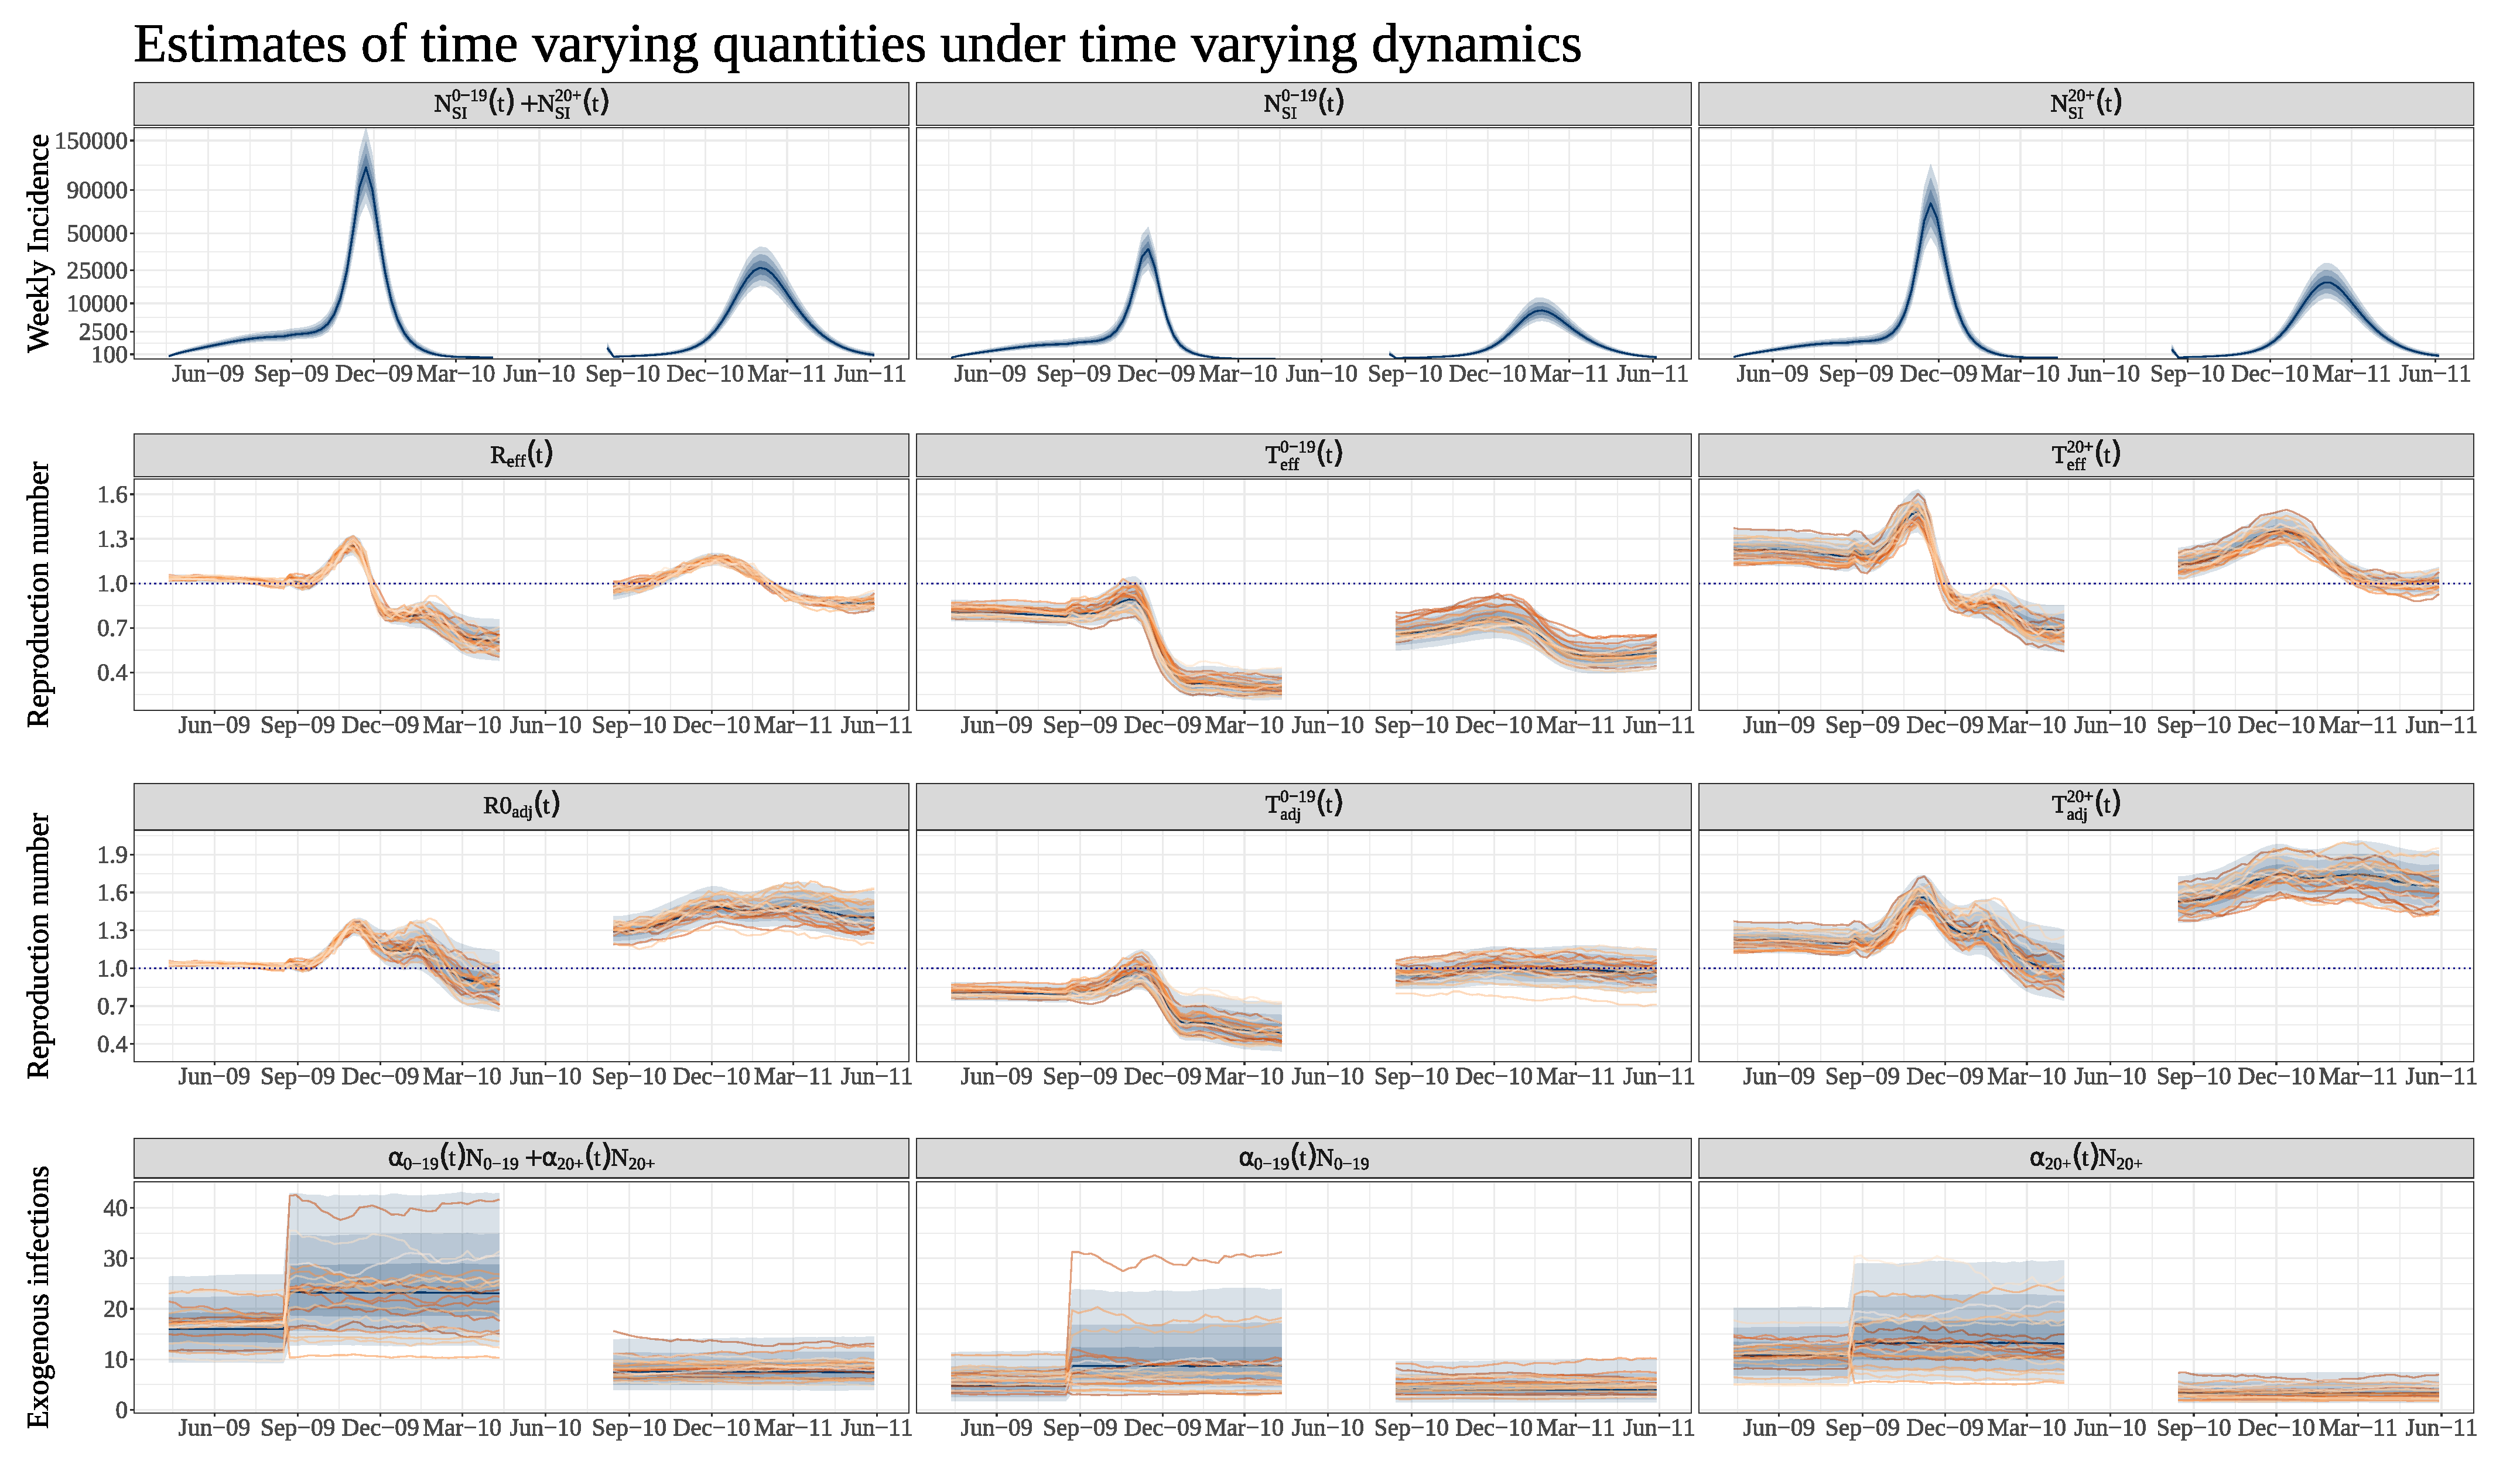
\includegraphics[width=0.95\linewidth]{figures/flu_rw_ode_timevarying_plots}
	\caption[Estimated A(H1N1) incidence, reproduction numbers, and rates of exogenous infection under time--varying dynamics.]{Posterior estimates of time--varying quantities under time--varying dynamics. Estimated incidence (top row), effective reproduction numbers (second row), vaccination adjusted basic reproduction numbers (third row), and exogenous infections (bottom row). $ N_{SI}^j(t), $ is the weekly incidence in age stratum $ j $, $ R_{eff}(t) $ and $ R_{adj}(t) $ are the effective and vaccination--adjusted basic reproduction numbers, $ T_{eff}^j(t) $ is the type reproduction number for stratum $ j $ (expected \# of secondary infections in all strata for a single infected in stratum $ j $), and $ \alpha_j(t) $ is the rate of exogenous infectious contacts for stratum $ j $.}
	\label{fig:flurwodetimevaryingplots}
\end{sidewaysfigure}

The mean infectious period of youths was slightly longer that of adults, 2.5 days (95\% BCI: 1.9 days, 3.5 days) compared with 2.1 days (1.8 days, 5.8 days), respectively. Published point estimates of the serial interval for A(H1N1)pdm09, which is the average time between an index case and a secondary case, and which we might expect to be a bit shorter than the mean infectious period, have mostly been in the 2--3.5 day range \cite{vink2014serial}. Immunity following infection was relatively long--lasting, although a sizable percentage of individuals who were infected lost immunity; 19\% (95\% BCI: 12\%, 28\%) of individuals who had become infected before the start of the second season had lost protection by the beginning of the second season, while the percentage of infected individuals who became infected over both seasons and lost immunity by the end of season two was 27\% (95\% BCI: 18\%, 38\%). The vaccine was estimated to be quite effective,  reducing the rate of infectious contact by 81\% (95\% BCI: 4\%, 46\%). 

\begin{sidewaystable}[htbp]
	\caption[Posterior estimates of SIRS model parameters for pandemic A(H1N1) influenza in Finland.]{Posterior medians (95\% Bayesian credible intervals) of SIRS model parameters for pandemic A(H1N1) influenza in Finland. The corresponding priors are given in Tables \ref{tab:flu_priors} and \ref{tab:flu_priors_const}.} 
	\label{tab:flu_param_ests}
	\centering\footnotesize
	\begin{tabular}{clrr}
		\hline
		&&\multicolumn{2}{c}{\textbf{Dynamics}}\\
		\cmidrule{3-4}\textbf{Parameter} & \textbf{Interpretation} & \textit{Time varying} & \textit{Piecewise homogeneous}\\
		\hline
		$ \psi_{Y,0} $ & Intrinsic $ R_0 $ for youths at epiweek 15, 2009  & 1.0 (0.99, 1.1) & 1.0 (0.95, 1.2)\\
		$ \psi_{Y,19} $ & Intrinsic $ R_0 $ for youths at epiweek 35, 2009 & 1.1 (1.0, 1.1) & 1.5 (1.1, 1.8)\\
		$ \psi_{Y,71}^{adj} $ & Vaccination adjusted intrinsic $ R_0 $ for youths at epiweek 33, 2010 & 1.2 (1.0, 1.3) & 1.2 (0.95, 1.5)\\
		$ \psi_{A,0} $ & Intrinsic $ R_0 $ for adults at epiweek 15, 2009  & 1.0 (1.0, 1.1) & 1.0 (0.94, 1.1)\\
		$ \psi_{A,19} $ & Intrinsic $ R_0 $ for adults at epiweek 35, 2009 & 1.0 (0.98, 1.1) & 1.1 (1.0, 1.2)\\
		$ \psi_{A,71}^adj $ & Vaccination adjusted intrinsic $ R_0 $ for adults at epiweek 33, 2010 & 1.3 (1.2, 1.5) & 1.4 (1.3, 1.6)\\
		$ 1/\mu_{Y} $ & Mean infectious period for youths (days) & 2.5 (1.9, 3.5) & 5.5 (3.5, 7.5)\\
		$ 1/\mu_A $ & Mean infectious period for adults (days) & 2.1 (1.8, 2.4) & 2.6 (2.2, 3.1)\\
		$ 1/\omega $ & Mean duration of immunity (years) & 3.6 (2.4, 5.8) & 4.5 (2.8, 7.3)\\
		$ \nu $ & 1 - VE for susceptibility & 0.19 (0.04, 0.54) & 0.05 (0.01, 0.19)\\
		$ s_Y $ & \% susceptible youths, $ S^{(u)}_Y(t_0) / N_Y $ & 0.28 (0.21, 0.36) & 0.34 (0.26, 0.42) \\
		$ s_A $ & \% susceptible adults, $ S_A^{(u)}(t_0) / N_A $ & 0.28 (0.21, 0.35) & 0.32 (0.24, 0.40) \\
		$ \rho_Y $ & Mean case detection rate for youths & 0.013 (0.01, 0.02) & 0.015 (0.01, 0.02)\\
		$ \rho_A $ & Mean case detection rate for adults & 0.008 (0.006, 0.01) & 0.0008 (0.006, 0.01)\\		
		$ 1/\sqrt{\phi_Y} $ & Negative binomial overdispersion for youths & 0.71 (0.55, 0.92) & 1.1 (0.86, 1.3)\\
		$ 1/\sqrt{\phi_A} $ & Negative binomial overdispersion for adults & 0.56 (0.37, 0.76) & 1 (0.82, 1.20)\\
		\hline
	\end{tabular}
\end{sidewaystable}

The effective reproduction numbers in the first season fell below one several months before the vaccination adjusted basic reproduction numbers. This suggests that the end of the first wave outbreak largely came about due to the depletion of susceptibles, rather than due to the aggressive vaccination campaign. Nevertheless, there is evidence to suggest that the vaccination campaign mitigated the severity of the epidemic. Table \ref{tab:flu_novacc_ests} presents naive estimates of the increases in incidence and attack rates by age stratum and season, which are obtained by setting vaccine coverage to zero and simulating outbreaks from the posterior. Without vaccination, we estimate that an additional 8.1\% (95\% PPI: 4.0\%, 12.5\%) of the population would have become infected over the course of both seasons. The vaccination campaign likely mitigated the severity of the second wave, in particular. We estimate that the attack rate would have been 1.3--fold (95\% PPI: 1.1, 1.5) higher in the first season, and 2.1--fold (95\% PPI: 1.4, 3.3) higher in the second season absent the effects of vaccination. 

In addition to mitigating the outbreak severity, we also find that the vaccination campaign may have delayed the second wave of the outbreak by roughly four months. Incidence peaked during the second season in late January to early February (posterior median: epiweek 6, 2011; 95\% BCI: epiweek 4, epiweek 7). Our model predicts that, absent vaccination, incidence would have peaked between the September and mid November (posterior median: epiweek 41, 2010; 95\% PPI: epiweek 38, epiweek 47). A similar finding was reported in \cite{shubin2016revealing}. We caution that this result should not be over--interpreted as it is most likely an artifact of the procedure used to predict the counterfactual outcomes. The per--contact infection rates at the start of each epoch are calibrated such that the effective reproduction numbers (\ref{eqn:Reff_t}), which account for vaccination, are roughly one (see Figure \ref{fig:flurwodetimevaryingplots}, second row). Setting vaccination to zero has the effect of artificially inflating the effective reproduction number, and hence the per--contact infection rate, by the fraction of the effective population size. Hence, the model mistakenly predicts that the epidemic takes off immediately in the third epoch.

We can make a rough adjustment to account for the artificial inflation in the FOI by rescaling the intrinsic reproduction numbers by the reduction in $ R_0 $ that would have been achieved with vaccination in the absence of any infections or recoveries. Let $ \psi_{j,\ell}^{adj} $ denote the vaccination adjusted reproduction number in week $ \ell $, which scaled as
\begin{equation}
\label{eqn:R0_adj}
\psi_{j,\ell}^{adj} = \psi_{j,\ell}\left (1 - P^v_j(t_\ell) + \nu P^v_j(t_\ell)\right ).\end{equation}
We set vaccination counts to zero as before and simulate outbreaks using the posterior distribution of the adjusted reproduction numbers. After adjustment, we predict that the overall attack rate would have been roughly 1.2--fold higher (95\% PPI: 1.1, 1.5) in the absence of vaccination, which is lower than the unadjusted estimate. We predict that the attack rates would have been roughly 1.2--fold higher (95\% PPI: 1.1, 1.3) in the first season, and 1.3--fold higher (95\% PPI: 1.0, 1.8) in the second season were it not for the vaccination campaign. We also predict that the second season would have peaked between late December and late February (posterior median: epiweek 2, 2011; 95\% PPI: epiweek 51, 2010, epiweek 9, 2011). Thus, after adjusting for the artificial inflation of contact rates, we do not find evidence to suggest that the second epidemic wave would have taken off in the late summer or early fall. 
 
\begin{table}[htbp]
	\caption[Naive predictions of incidence and attack rates in the absence of vaccination.]{Naive predictions of incidence and attack rates in the absence of vaccination. Increases in cumulative incidence (thousands), absolute percent increase, and relative fold--increase in attack rates without vaccination by season and age stratum.}
	\label{tab:flu_novacc_ests}
	\centering\footnotesize
	\begin{tabular}{lrrr}
		\hline
		&\multicolumn{3}{c}{\textit{Season 1}}\\
		\cmidrule{2-4} 
		 & Incidence ($ \times10^3 $) & Attack rate (Abs. \% diff.) & Attack rate (Fold--change) \\
		 \hline
		 Ages 0-19 & 45.4 (21.4, 71.8) & 3.7 (1.7, 5.9) & 1.3 (1.1, 1.4)\\
		 Ages 20+ & 107 (51.9, 162) & 2.6 (1.3, 3.9) & 1.3 (1.1, 1.5)\\
		 All ages & 154 (74.9, 226) & 2.9 (1.4, 4.2) & 1.3 (1.1, 1.5)\\
		 \hline
		 &&&\\
		 &\multicolumn{3}{c}{\textit{Season 2}}\\
		 \cmidrule{2-4} 
		 &Incidence ($ \times10^3 $) & Attack rate (Abs. \% diff.) & Attack rate (Fold--change) \\
		 \hline
		 Ages 0-19 & 66.1 (25.3, 125) & 5.4 (2.1, 10.2) & 2.0 (1.3, 3.1)\\
		 Ages 20+ & 202 (85.9, 359) & 4.9 (2.1, 8.7) & 2.2 (1.4, 3.5)\\
		 All ages & 272 (121, 456) & 5.1 (2.3, 8.5) & 2.1 (1.4, 3.3)\\
		 \hline
		  &&&\\
		 &\multicolumn{3}{c}{\textit{Both seasons}}\\
		 \cmidrule{2-4} 
		 &Incidence ($ \times10^3 $)& Attack rate (Abs. \% diff.) & Attack rate (Fold--change) \\
		 \hline
		 Ages 0-19 & 113 (50.7, 192) & 9.3 (4.1, 15.7) & 1.5 (1.2, 1.9)\\
		 Ages 20+ & 314 (156, 509) & 7.6 (3.8, 12.3) & 1.6 (1.3, 2.1)\\
		 All ages & 432 (216, 668) & 8.1 (4, 12.5) & 1.6 (1.3, 2.0)\\
		\hline
		\hline
	\end{tabular}
\end{table}

\begin{table}[htbp]
	\caption[Adjusted estimates of predicted incidence and attack rates in the absence of vaccination.]{Effects of vaccination adjusted for artificial inflation of reproduction numbers in the absence of vaccination. Increases in cumulative incidence (thousands), absolute percent increase, and relative fold--increase in attack rates without vaccination by season and age stratum.}
	\label{tab:flu_novacc_adj}
	\centering\footnotesize
	\begin{tabular}{lrrr}
		\hline
		&\multicolumn{3}{c}{\textit{Season 1}}\\
		\cmidrule{2-4} 
		& Incidence ($ \times10^3 $) & Attack rate (Abs. \% diff.) & Attack rate (Fold--change) \\
		\hline
		Ages 0-19 & 34 (16, 52) & 2.8 (1.3, 4.3) & 1.2 (1.1, 1.3)\\
		Ages 20+ & 75 (36, 110) & 1.8 (0.9, 2.7) & 1.2 (1.1, 1.4)\\
		All ages & 110 (54, 160) & 2 (1.0, 3.0) & 1.2 (1.1, 1.3)\\
		\hline
		&&&\\
		&\multicolumn{3}{c}{\textit{Season 2}}\\
		\cmidrule{2-4} 
		&Incidence ($ \times10^3 $) & Attack rate (Abs. \% diff.) & Attack rate (Fold--change) \\
		\hline
		Ages 0-19 & 12 (-2.5, 37) & 1.0 (-0.2, 3.1) & 1.2 (0.97, 1.6)\\
		Ages 20+ & 52 (2.7, 140) & 1.3 (0.1, 3.4) & 1.3 (1, 2)\\
		All ages & 65 (3.3, 170) & 1.2 (0.1, 3.3) & 1.3 (1, 1.8)\\
		\hline
		&&&\\
		&\multicolumn{3}{c}{\textit{Both seasons}}\\
		\cmidrule{2-4} 
		&Incidence ($ \times10^3 $)& Attack rate (Abs. \% diff.) & Attack rate (Fold--change) \\
		\hline
		Ages 0-19 & 47 (18, 84) & 3.8 (1.5, 6.9) & 1.2 (1.1, 1.4)\\
		Ages 20+ & 130 (48, 240) & 3.1 (1.2, 5.7) & 1.2 (1.1, 1.5)\\
		All ages & 180 (70, 310) & 3.3 (1.3, 5.9) & 1.2 (1.1, 1.5)\\
		\hline
	\end{tabular}
\end{table}

The posterior predictive distributions in Figure \ref{fig:flupostpredsrwode} suggest that the model does a better job reconstructing the second epidemic season than the first, particularly among individuals ages 0--19. The model appears to underestimate the peak of the outbreak among youths in the first season. One possibility is that heterogeneity in detection rates is confounding our estimates of the dynamics. In their analysis of this data, \cite{shubin2016revealing} estimated that detection was positively associated with incidence, and it is known that heterogeneity in detection rates can confound estimates of outbreak dynamics \cite{caley2008quantifying,glass2011estimating,white2010reporting}. Another possibility is that the assumption of constant within--epoch variance of log differences of time--varying reproduction numbers is leading to underestimation of the peak reproduction numbers. It is challenging to tune the GMRFs so that they capture changes in the dynamics over time but are not so flexible that we lose identifiability. It is possible that introducing additional changepoints in the time--varying dynamics, or using a model that allows for non--constant variance in the GMRF increments might alleviate this problem. Finally, it is possible that dichotomizing the population into two age strata does not adequately capture the age structure in contact patterns, incidence, and vaccination. A more granular model with additional age strata might be better able to capture the dynamics of the outbreak.

\begin{figure}[htbp]
	\centering
	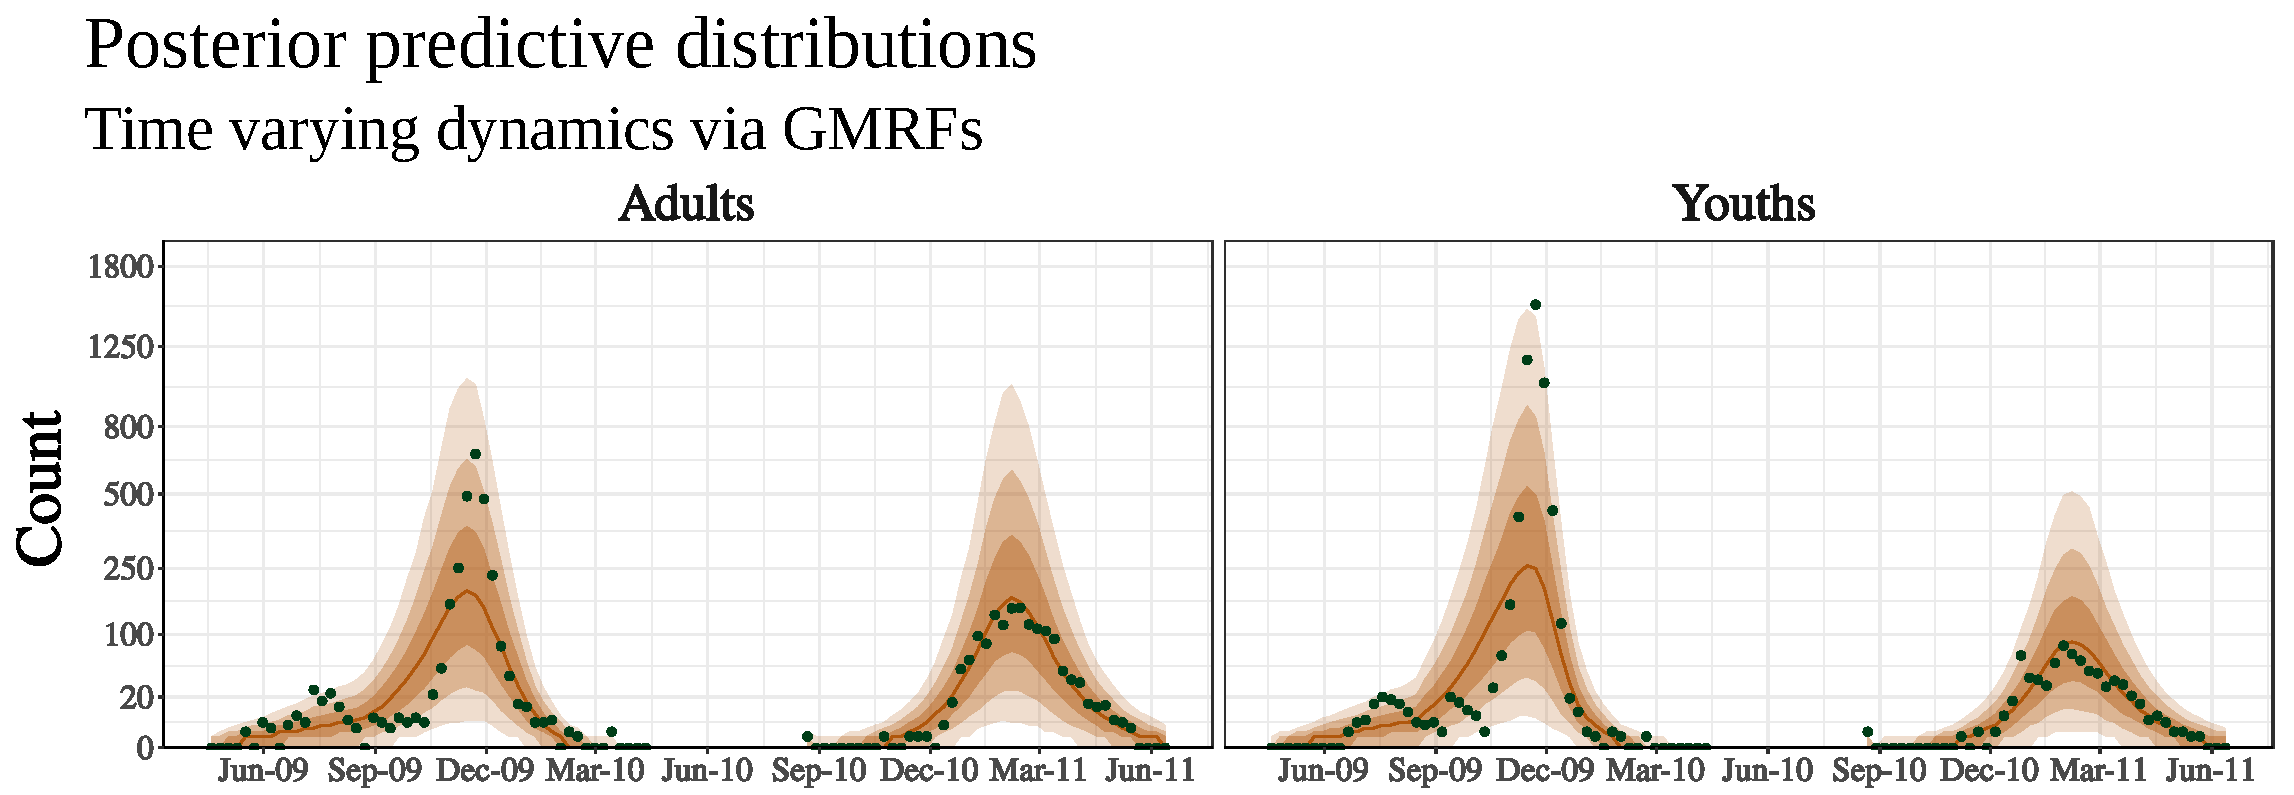
\includegraphics[width=\linewidth]{figures/flu_postpreds_rw_ode}
	\caption{Posterior predictive distributions of a stratified SIRS ODE model with time--varying dynamics for A(H1N1)pdm09 in Finland.}
	\label{fig:flupostpredsrwode}
\end{figure}

\subsection{Comparison with Piecewise Homogeneous Dynamics}
\label{subsec:flu_res_homog}

For comparison, we fit a model where the outbreak dynamics were piecewise homogeneous in each epoch. The basic reproduction numbers and rates of exogenous infection were estimated for each of the three epochs, but unlike the previous model were held constant within each epoch. The remaining aspects of the model structure and emission distributions were similar to the time--varying model. Estimates of incidence and attack rates are presented in Table \ref{tab:flu_attack_rates}, posterior distributions of time--varying quantities are presented in Figure \ref{fig:fluconstodetimevaryingplots}, and posterior estimates of model parameters are summarized in Table \ref{tab:flu_param_ests}. 

\begin{sidewaysfigure}[htbp]
	\centering
	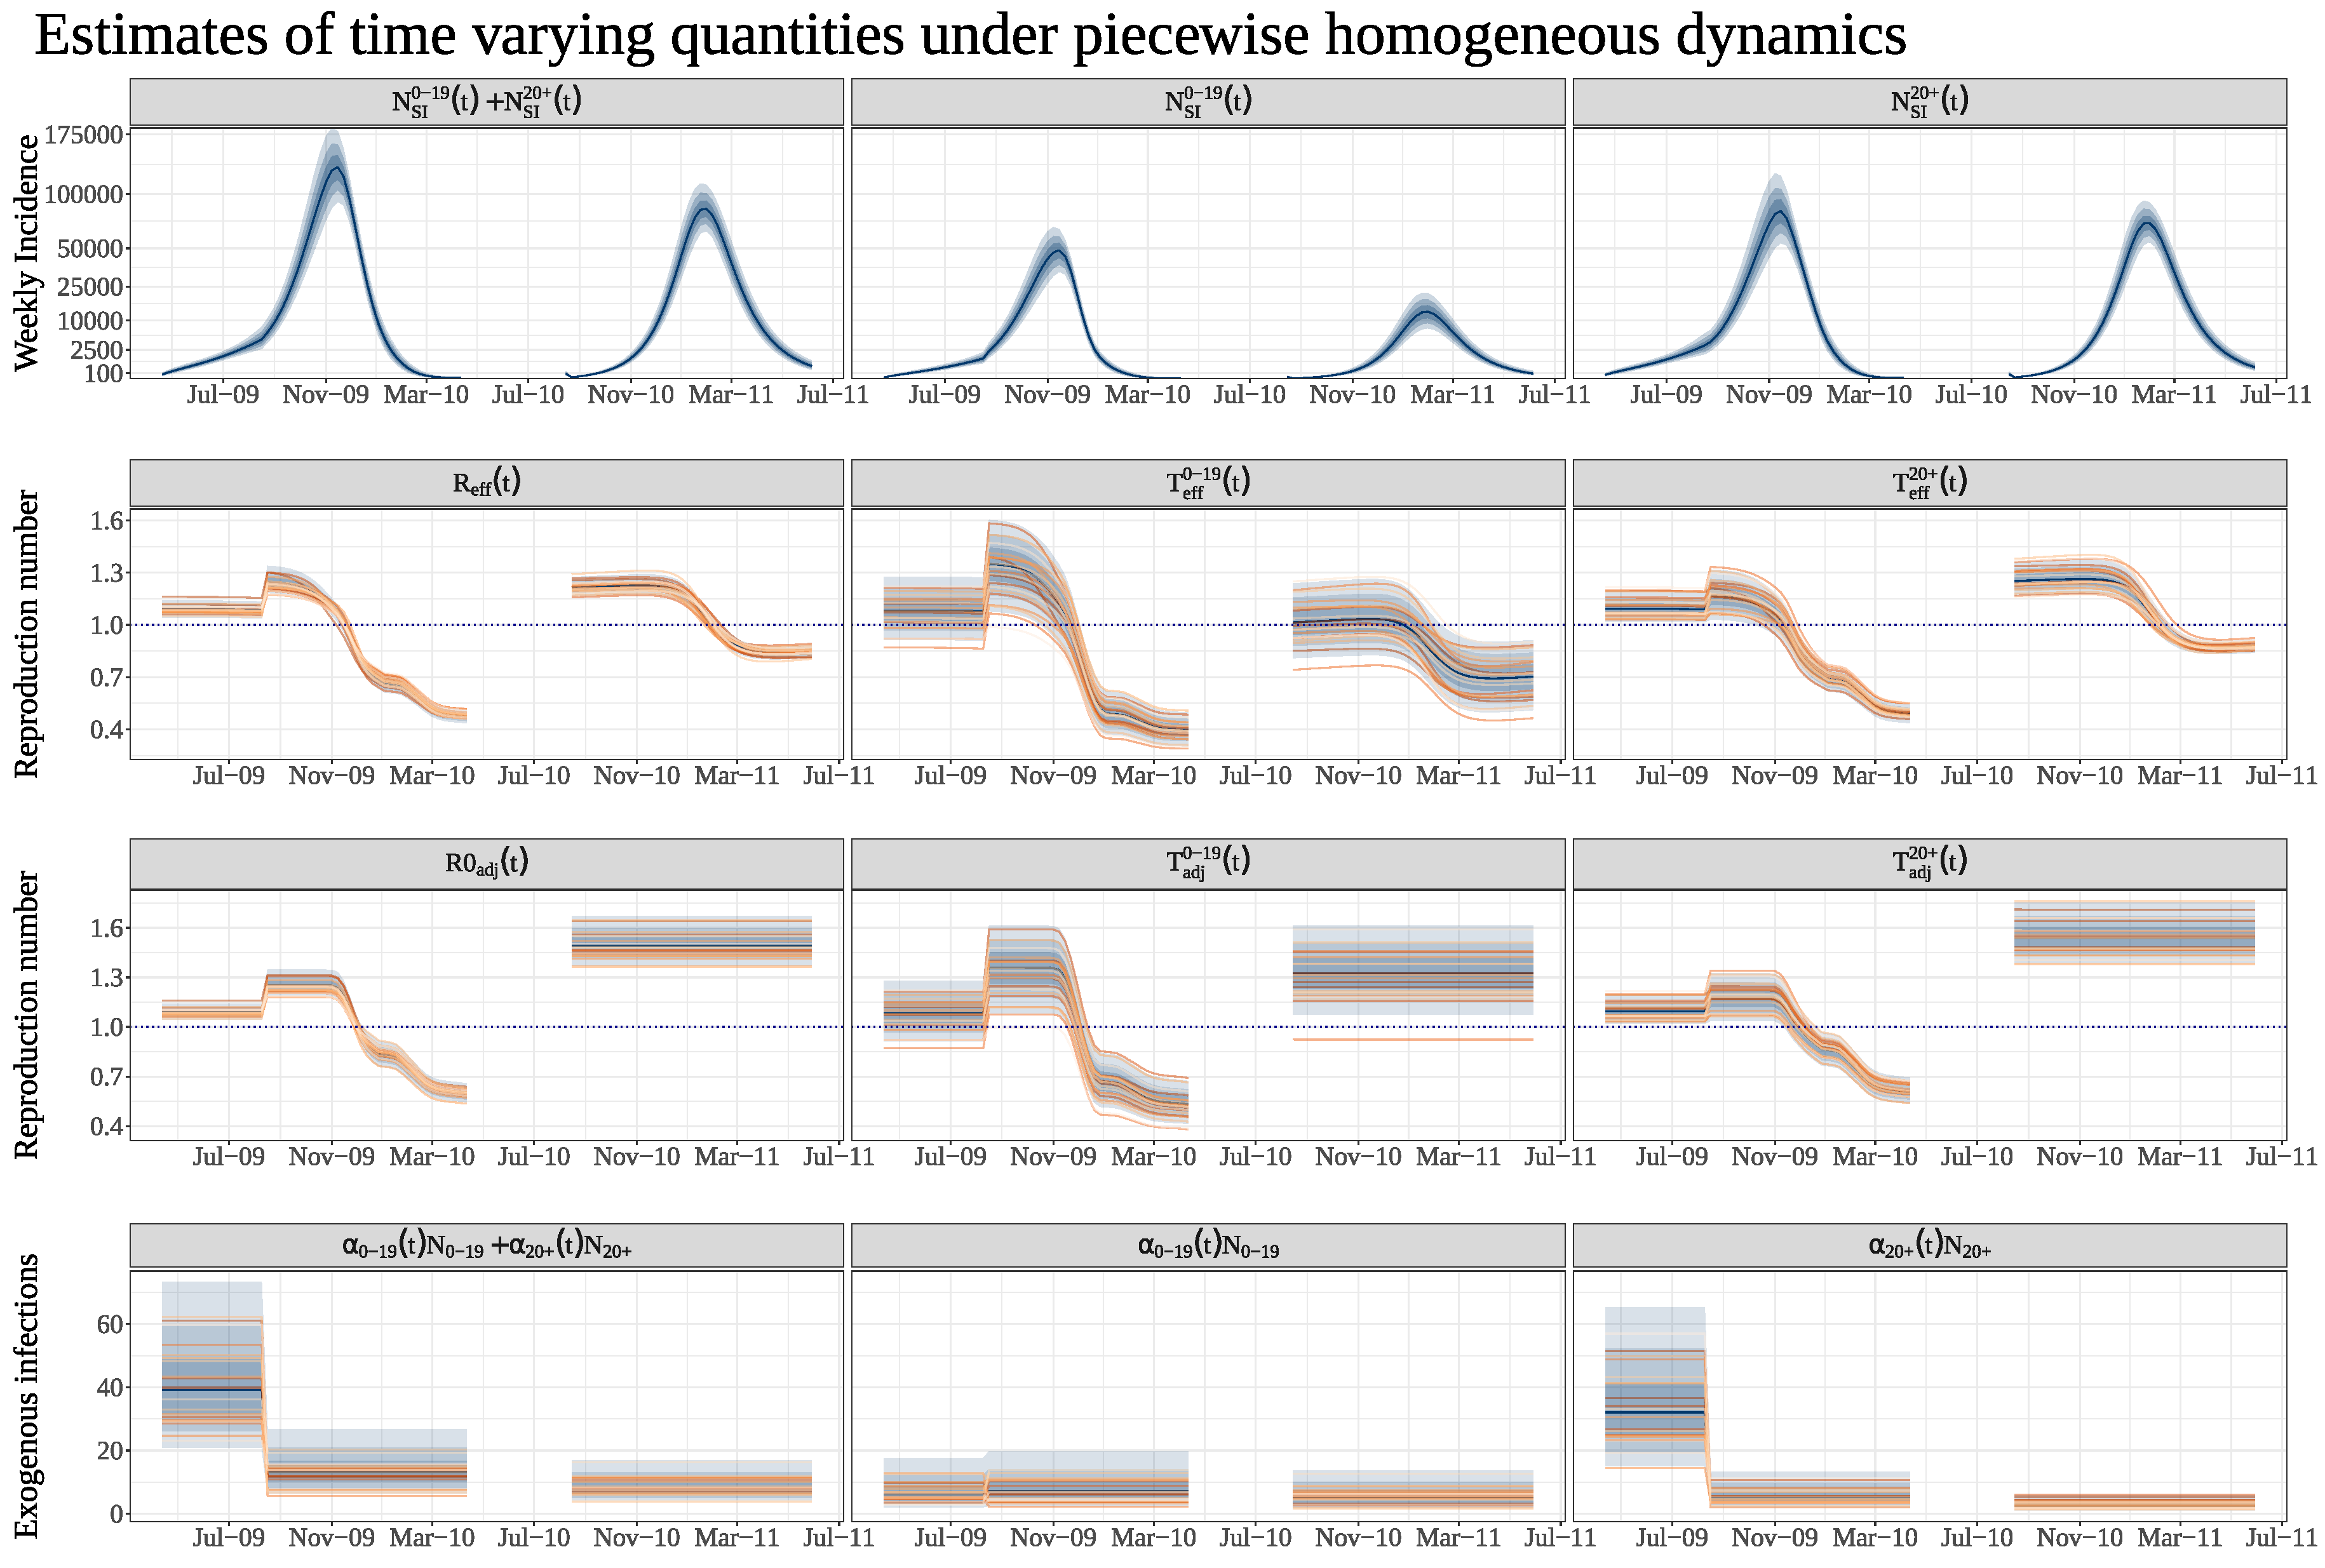
\includegraphics[width=0.95\linewidth]{figures/flu_const_ode_timevarying_plots}
	\caption[Estimated A(H1N1) incidence, reproduction numbers, and rates of exogenous infection under piecewise homogeneous dynamics.]{Posterior estimates of time--varying quantities under piecewise homogeneous dynamics. Estimated incidence (top row), effective reproduction numbers (second row), vaccination adjusted basic reproduction numbers (third row), and exogenous infections (bottom row). $ N_{SI}^j(t), $ is the weekly incidence in age stratum $ j $, $ R_{eff}(t) $ and $ R_{adj}(t) $ are the effective and vaccination--adjusted basic reproduction numbers, $ T_{eff}^j(t) $ is the type reproduction number for stratum $ j $ (expected \# of secondary infections in all strata for a single infected in stratum $ j $), and $ \alpha_j(t) $ is the rate of exogenous infectious contacts for stratum $ j $.}
	\label{fig:fluconstodetimevaryingplots}
\end{sidewaysfigure}

Attack rates under piecewise homogeneous dynamics were slightly lower than under time--varying dynamics (Table \ref{tab:flu_attack_rates}). Average dwell times in the infected and recovered states were longer, and the reduction in the rate of infectious contact for vaccinated individuals was substantially greater under piecewise homogeneous dynamics. Two striking differences in the time--varying aspects of the piecewise homogeneous model are in the rates of exogenous infection in each epoch, and the contributions of youths and adults to the force of infection. The highest rates of exogenous infectious contact under piecewise homogeneous dynamics are in the first epoch in the adult sub--population. This might seem paradoxical, but in fact it is an artifact of the inability of the piecewise homogeneous model to accommodate the sub--exponential dynamics that were observed in the first five months of the modeling period. It is somewhat more surprising that the piecewise homogeneous model suggests that transmission from infectious contact with youths alone could possibly have sustained the outbreak in the first epidemic season, and also possibly in the second season. Youths comprised roughly 20\% of the population and only 15\% of the contacts made by adults. Hence, it seems dubious that the effective type reproduction numbers for youths in the first season, and possibly in the second epidemic season, would have been above one. 

Unsurprisingly, the GMRF model is much better able to capture the shape to the outbreak than is the model with piecewise homogeneous dynamics. The posterior predictive distribution indicates that the model has particular difficulty modeling the first wave of the outbreak and predicted that incidence begin to increase exponentially much sooner than was observed. It is possible that delaying the second modeling epoch several weeks to, say, late September could mitigate this behavior. Directly comparing the posterior predictive p-values and posterior predictive interval widths with those of the GMRF model shows that the piecewise homogeneous produces substantially wider predictive intervals with no obvious improvement in accuracy (Figure \ref{fig:flu_rw_const_ppicomp}).

\begin{figure}[htbp]
	\centering
	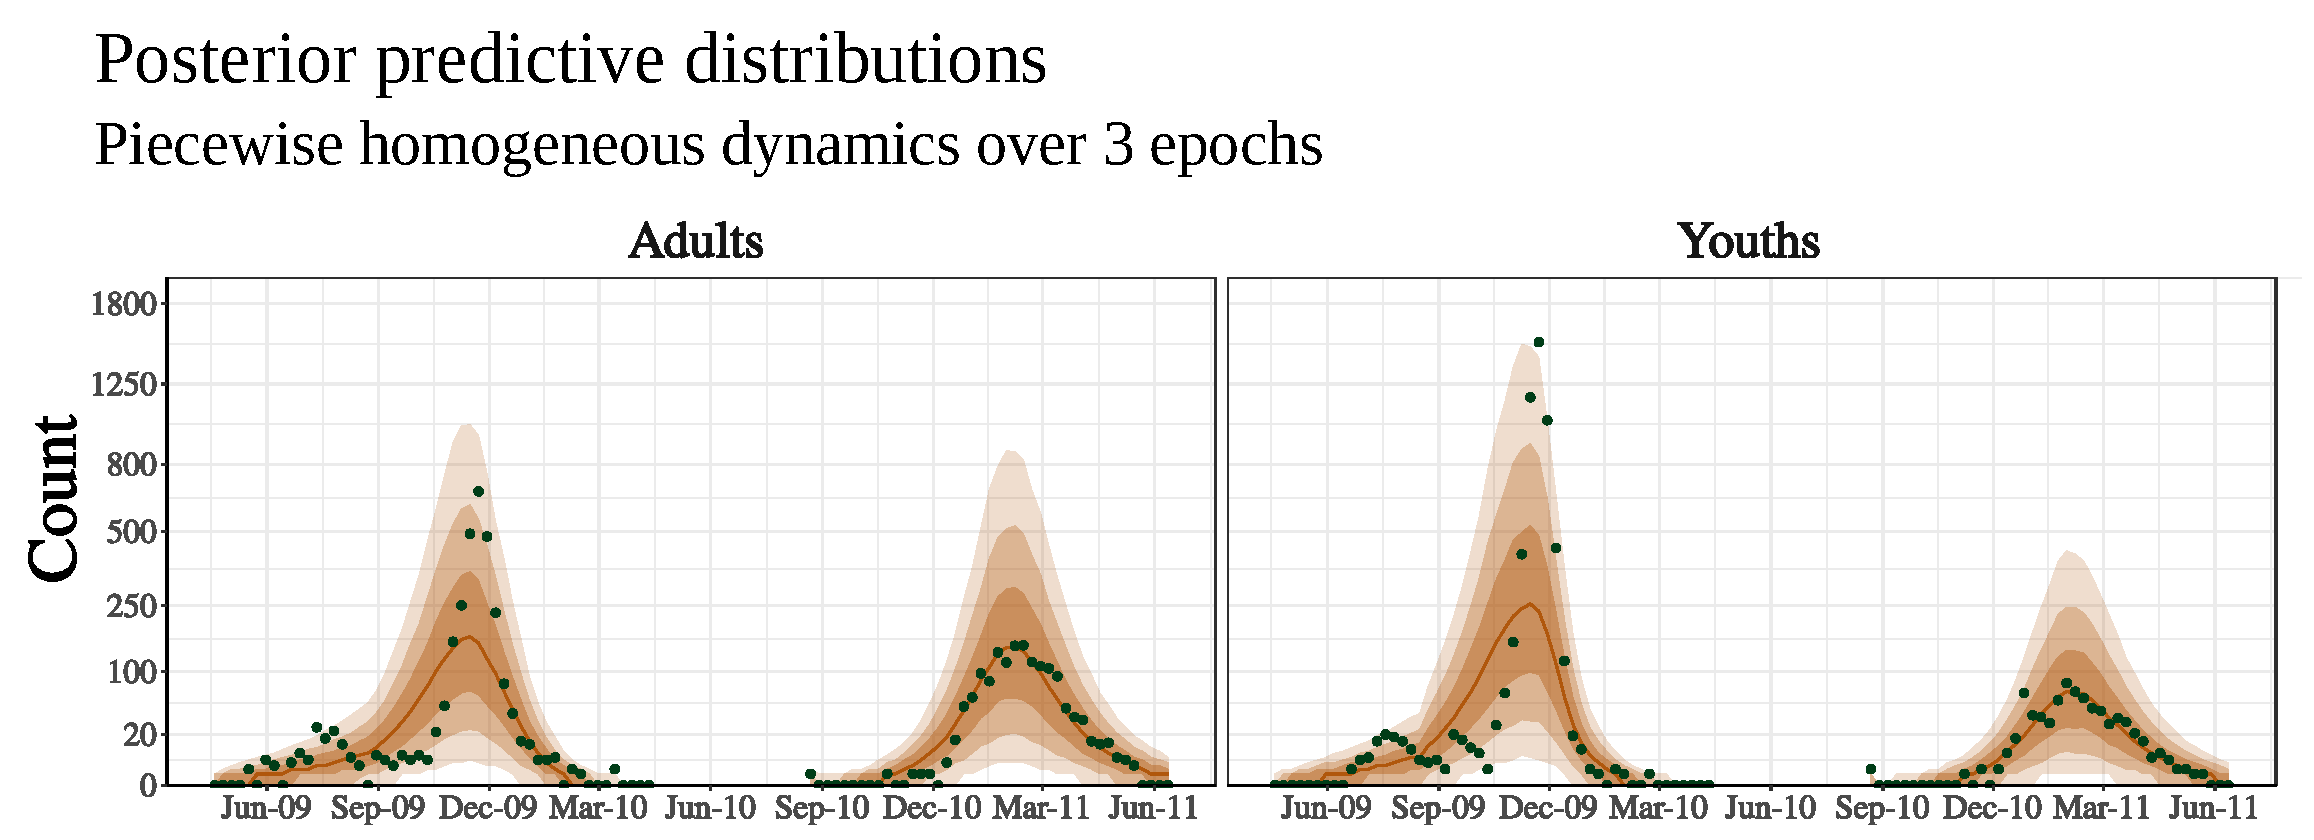
\includegraphics[width=\linewidth]{figures/flu_postpreds_const_ode}
	\caption{Posterior predictive distributions of a stratified SIRS ODE model with piecewise homogeneous dynamics over three epochs for A(H1N1)pdm09 in Finland.}
	\label{fig:flupostpredsconstode}
\end{figure}

\begin{figure}[htbp]
	\centering
	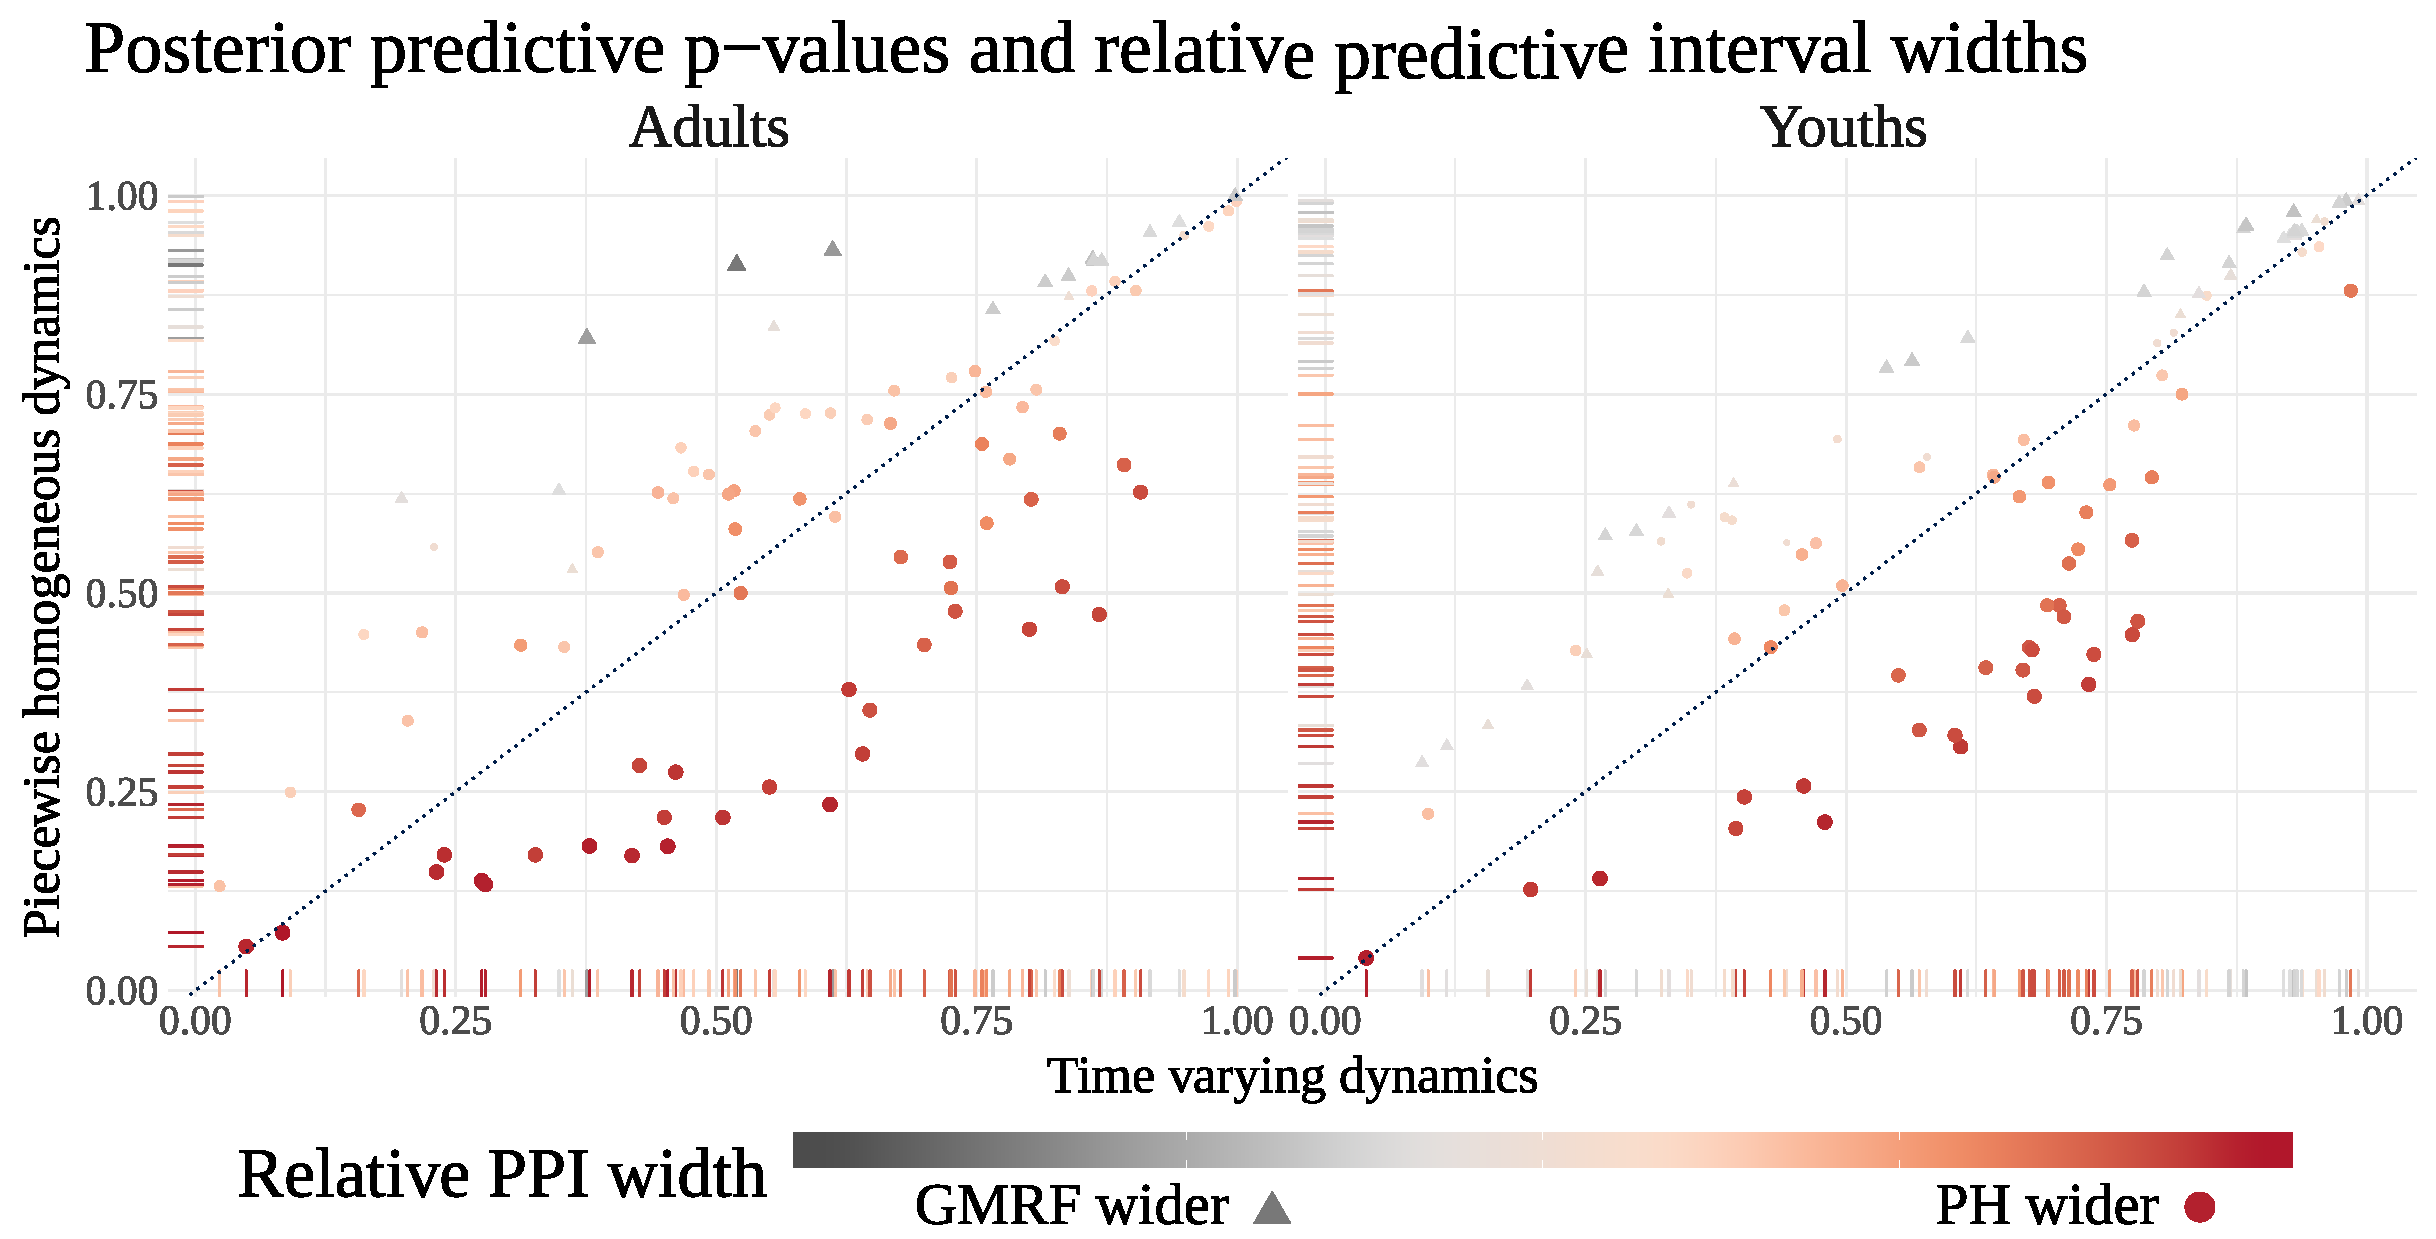
\includegraphics[width=\linewidth]{figures/flu_rw_const_ppicomp}
	\caption[Comparison with posterior predictive p-values and relative predictive interval widths for SIRS models with time--varying and piecewise homogeneous dynamics.]{Comparison of models with time--varying (GMRF) and piecewise homogeneous (PH) dynamics using posterior predictive p-values (PPPs) and relative posterior predictive interval (PPI) widths. Each point corresponds to the observed incidence in a given week. The X--Y coordinates give the PPPs under time--varying and piecewise homogeneous dynamics, respectively. The size and color of each point corresponds to the relative PPI width, computed as $ (\widehat{\sigma}_{post,\ell}^{GMRF} - \widehat{\sigma}_{post,\ell}^{PH})/\widehat{\sigma}_{post,\ell}^{GMRF} $, and the sign of the relative width is further emphasized by the shape of the point. Red dots indicate that PPIs under piecewise homogeneous dynamics are wider and grey triangles indicate that PPIs under time--varying dynamics are wider.}
	\label{fig:flu_rw_const_ppicomp}
\end{figure}

\section{Discussion}
\label{sec:flu_discussion}

We began this chapter by highlighting the importance of allowing for the possibility that transmission dynamics might change over time. We used the LNA framework developed in Chapter \ref{chap:lna_for_sems} to fit an SIRS model with time--varying dynamics, where time--varying reproduction numbers were flexibly modeled using a Gaussian Markov random field that penalized the magnitude of week--to--week changes in basic reproduction numbers. We compared the results to those obtained using an SIRS model with time homogeneous dynamics and found that the model with time homogeneous dynamics, which unlike the flexible model was unable to accurately reconstruct the unobserved incidence, the time--varying aspects of the transmission dynamics, or even static model parameters.

We then developed an age--vaccination stratified SIRS model for the spread of pandemic A(H1N1) influenza in Finland over two epidemic waves. We allowed for the possibility that various static and temporal aspects of transmission dynamics were different in youths and adults, and incorporated information about the contact patterns between individuals of different ages. The model also incorporated uncertainty about vaccine efficacy and loss of immunity, rather than fix these quantities as was done in previous analyses \cite{shubin2016revealing}. Critically, the model allowed for time--varying dynamics within each of three epochs by assigning GMRF shrinkage priors to the intrinsic reproduction numbers and rates of exogenous infection in each age stratum. This enabled the model to greatly outperform a piecewise homogeneous model that, in some aspects, yielded somewhat unreasonable estimates. 

Due to the complexity of the model, we opted to use the ODE representation in fitting it. The lower computational burden involved in fitting the ODE model allowed us to more quickly iterate through various  parameterizations and to explore the effects of different priors, and in particular of alternative GMRF formulations. Run times for the model were on the order of 1--2 hours. We are confident that the model could also be fit using the LNA with some additional effort. One future line of inquiry is in comparing the statistical performance of models with varying dynamics fit via the LNA and ODE. It would be useful to know the extent to which randomness in the latent epidemic process and the time--varying aspects of its dynamics are separately identifiable from incidence data, especially if there are situations where the latent process and its dynamics are not separately identifiable.

A strength of the analysis is that the two epidemic seasons were jointly modeled along with the pre--epidemic and inter--season periods. This provides us with a principled structure for incorporating uncertainty about the state of the population at the start of each epidemic wave. This is critical to making accurate inferences about the true incidence and model dynamics, especially during the second epidemic season where the dynamics inherently depend on the attack rate during the first season and the fraction of individuals who lost immunity during the inter--season period. Moreover, the assumption that vaccination was independent of the infection process implies that the distribution of vaccine doses at the beginning of the second season is also tied up with the attack rate in the first season (e.g., a low attack rate in the first season implies that there are many vaccinated susceptibles to start the second season). For these reasons, it is important to jointly model both epidemic seasons.

There are a few aspects of the analysis that we point to as weaknesses and that should be improved in future work. First, it is important to recognize that our estimates of the cumulative incidence are predicated on the correctness of our assumptions about the effective population size. In a supplementary analysis, we found that centering the prior for the susceptible fraction of youths at 50\% instead of 25\%, while holding the prior for the susceptible fraction of adults constant, yielded estimates of cumulative incidence among youths that were roughly double the estimates reported in this chapter (Section \ref{subsec:flu_highsusc_sensitivity}). Frankly, it is doubtful that the reporting rates and true incidence can be unambiguously estimated from partially observed incidence data without strong assumptions when detection rates are low and in the absence of prevalence data to anchor estimates of the total outbreak size. We attempted to set the priors for the effective population size in a principled way based on known final size relations for SIR models combined with, what we felt, were reasonable assumptions about detection rates (Section \ref{subsubsec:flu_effpop_priors}). Our estimates are also in line with estimated attack rates for A(H1N1)pdm09 in Finland \cite{cuesta2016pandemic,shubin2014estimating,shubin2014estimating} and in other settings \cite{dawood2012estimated,opatowski2011transmission,steens2011age}. In this chapter, we did not incorporate data on severe cases and hospitalizations, which would help to calibrate inference of the total outbreak size, assuming that the case--hospitalization ratio is stable. This data is available and was previously analyzed in \cite{shubin2016revealing}. 
 
Another aspect of the model that could be improved is the coarseness of the age structure. We dichotomized the population for simplicity and computational expediency. However, further stratifying the population would allow us to more faithfully represent age structure in contact rates, vaccination, and transmission dynamics. We suggest that, at a minimum, individuals age 0--4 could be split from individuals age 5--19, and that individuals of ages 65+ be split from other adults based on differences in the timing and coverage of vaccinations, observed patterns in attack rates, and contact patterns. 